\providecommand{\main}{../../..}
\documentclass[\main/dresen_thesis.tex]{subfiles}

\begin{document}
  Cobalt ferrite nanoparticles are nowadays routinely synthesized following methods such as co-precipitation \cite{Fried_2001_Order}, sol-gel \cite{Niederberger_2009_Metal}, micro emulsions \cite{Pillai_1996_Synth}, or thermal decomposition.
  For thermal decomposition, one can further differentiate between hot-injection \cite{Hyeon_2003_Chemi} and heating up methods \cite{Embden_2015_TheHe}.
  Where the first promises monodisperse nanoparticles by keeping the nucleation time period of the synthesis short, the latter is especially promising in being scaleable and highly controllable \cite{Park_2004_Ultra}.
  The heating up method is used extensively in this work to synthesize nanocubes and nanospheres of cobalt ferrite and iron oxide and is further elaborated in the following.

  A popular heating up route to synthesize nanoparticles is to first prepare a metal oleate precursor from metal salts, which is subsequently slowly heated above it's decomposition temperature in a high-boiling solvent, where it is aged in the presence of oleic acid and additional reagents to direct the growth and shape.
  For example, the shape of cobalt ferrite nanoparticles can be tuned by adding sodium oleate as precursor before the heating up process.
  The sodium oleate attaches to the (100) facets of forming nanocrystals and fosters the growth along the [111] direction of the crystal \cite{Bao_2009_Forma}.
  By tuning the ratio of sodium oleate to the oleate precursor and adjusting the aging time, this process allows to go from nanospheres over nanocubes to star-shaped nanoparticles.
  Wetterskog \etal extensively studied the formation of maghemite nanospheres and nanocubes, following the same route without cobalt oleate in the synthesis \cite{Wetterskog_2014_Preci, Wetterskog_2013_Anoma}, and found that due to the reducing environment a w\"ustite core is first formed and only by post-synthesis oxidation a maghemite shell is obtained.
  The same can be observed for the synthesis of cobalt ferrite nanoparticles from metal oleates \cite{Bodnarchuk_2009_Excha}, which explains in both cases the low degree of magnetism that is often observed in literature from such synthesis as w\"ustite is paramagnetic at room temperature and antiferromagnetic below $203 \unit{K}$.
  Through forced oxidation after the synthesis the magnetic properties can be enhanced especially for iron oxide nanoparticles \cite{Wetterskog_2013_Anoma}.
  However, cobalt ferrite provides a high oxygen diffusion barrier \cite{Chen_2015_Synth} and it is technically harder to oxidize cobalt ferrite nanoparticles completely without destroying the surfactant shell irreversibly.

  An alternative heating up synthesis that results in strongly magnetic nanoparticles with pure phase directly is achieved by the thermal decomposition of metal acetylacetonates in a high boiling solvent such as dibenzyl ether with the presence of oleic acid or oleylamine \cite{Sun_2002_SizeC, Wu_2014_Monol}.
  Again the addition of sodium oleate leads to the formation of nanocubes, such as in the oleate synthesis route, when the amount is tuned to the oleic acid content and aging time.
  However, this synthesis is in general difficult to control and scale partly due to the production of acetone during the synthesis that leads to small but violent explosions at elevated temperatures within the solution.
  Often the shape of the nanoparticles from this synthesis route is less uniform in comparison to the oleate synthesis route and a lot of fine-tuning and care has to be taken to obtain a homogeneous batch of nanoparticles that can be used for self-assembly experiments.

  In the following, the preparation of cobalt ferrite nanocubes following both routes is presented and the obtained nanoparticles are characterized similar to \refch{ch:looselyPackedNS}.
  The synthesis and characterization of iron oxide (maghemite/magnetite) nanocubes following the oleate route on the other hand is presented in \refch{ch:colloidalCrystals} for the framework of producing colloidal crystals.

  \subsection{Synthesis from Metal Oleates and Acetylacetonates}\label{sec:monolayers:nanoparticle:synthesisOleatesAcAc}
    \subsubsection{Preparation of Cobalt Ferrite Oleate}
      In the first presented protocol to synthesize cobalt ferrite nanoparticles, a cobalt and iron oleate mixture is prepared as first step.
      For this purpose a clear solution of sodium oleate is prepared by dissolving $96 \unit{mmol}$ of \ch{NaOH} in $20 \unit{mL}$ of each \ch{H2O} and \ch{EtOH} and subsequently adding drop wise $96 \unit{mmol}$ of oleic acid under constant stirring.
      Then $12 \unit{mmol}$ of \ch{CoCl2 * 6 H2O} and $24 \unit{mmol}$ of \ch{FeCl3 * 6 H2O} are dissolved in $5 \unit{mL}$ \ch{H2O} and $15 \unit{mL}$ \ch{EtOH} each and added to the solution.
      After addition of $80 \unit{mL}$ \ch{H2O} and \ch{EtOH} each, as well as $160 \unit{mL}$ n-hexane, the mixture is held at reflux ($60 \unit{^\circ C}$) for $4 \unit{h}$ under constant strong magnetic stirring.
      Once the mixture is cooled back to room temperature, it is washed three times in a separatory funnel with $30 \unit{mL}$ \ch{H2O} each to remove superfluous \ch{NaCl}.
      The remaining n-hexane, ethanol and water is removed using a rotary evaporator.
      In the end, approximately $32 \unit{g}$ of a dark red and highly viscous metal oleate complex is obtained, which is then ready to be used for the nanoparticle synthesis.

    \subsubsection{Preparation of Nanocubes from Oleate}
      To prepare nanoparticles, $10 \unit{mmol}$ of the cobalt ferrite oleate is dissolved in $50 \unit{mL}$ 1-octadecene within a $250 \unit{mL}$ three-neck round-bottom flask.
      To obtain cubically shaped nanoparticles, sodium oleate is prepared separately by dissolving $2.5 \unit{mmol}$ \ch{NaOH} in $10$ drops of \ch{H2O} and \ch{EtOH} and adding $2.5 \unit{mmol}$ of oleic acid drop wise while ultra sonificating the mixture.
      The sodium oleate is added to the dissolved oleate together with additional $2.5 \unit{mmol}$ oleic acid.
      The mixture is heated and held at $150 \unit{^\circ C}$ for one hour under constant magnetic stirring until all water and ethanol is evaporated.
      A fractionating column is put on the round-bottom flask and nitrogen is gently bubbled into the mixture.
      Using a temperature controller, the mixture is heated to reflux at approximately $315 \unit{^\circ C}$ with a gradient of $2.5 \unit{^\circ C min^{-1}}$, where it is held for $30 \unit{min}$.
      After cooling the reaction naturally to room temperature, the particles are precipitated with \ch{EtOAc} and \ch{EtOH}, centrifuged at $8000 \unit{rpm}$ and redispersed in n-hexane until the supernatant is clear.
      In the last step the mixture is centrifuged without adding \ch{EtOAc}/\ch{EtOH} and the supernatant fluid is taken as dispersion, where as the precipitate is thrown away as being unstable.
      This synthesis yields approximately $500 \unit{mg}$ nanocubes (yield $\approx 20 \%$) and is referred to in the following as Ol-CoFe-C.


    \subsubsection{Preparation of Nanocubes from Acetylacetonates}
      To synthesize nanocubes from acetylacetonates, $0.52 \unit{mmol}$ of \ch{Co(acac)2}, $0.8 \unit{mmol}$ of \ch{Fe(acac)3}, $3 \unit{mmol}$ of freshly prepared sodium oleate and $3 \unit{mmol}$ of oleic acid are diluted in $10 \unit{mL}$ of dibenzyl ether in a $50 \unit{mL}$ three-neck round-bottom flask.
      The mixture is heated to $120 \unit{^\circ C}$ and held here for $1 \unit{h}$.
      After putting a fractionating column on the round-bottom flask, a temperature controller is used to heat the mixture to reflux at about $290 \unit{^\circ C}$ with a heating rate of $5 \unit{^\circ C min^{-1}}$.
      During the synthesis, nitrogen is blown gently over the solution all the time to form an inert blanket and the solution is magnetically stirred.
      After cool down, the product is transferred with n-hexane to centrifugal tubes and precipitated with \ch{EtOH}.
      After centrifugation at $8500 \unit{rpm}$ the supernatant is thrown away and the precipitate is redispersed with n-hexane.
      This procedure is repeated three times and in the last step the precipitate is dispersed in n-hexane without precipitating it again.
      After a final centrifugation at $8500 \unit{rpm}$ the supernatant is kept as dispersion and the rest thrown away.
      The synthesis yields approximately $50 \unit{mg}$ nanocubes (yield $\approx 45 \%$) and is referred to in the following as Ac-CoFe-C.

  \subsection{Structural \& Magnetic Characterization of the Nanocubes}
  \label{sec:monolayers:nanoparticle:structuralCharacterization}
    After synthesis, transmission electron microscopy (TEM) is used to visually characterize a sample of the prepared dispersion and validate the structural quality of the batch.
    The exemplary micrograph shown in \reffig{fig:monolayers:nanoparticle:tem} reveal that both procedures result in nanocubes.
    The average particle size and size distribution of the particles is estimated from TEM by fitting the log-normal distribution described in \refeq{eq:looselyPackedNP:nanoparticle:lognormalDist}.
    The particles from the metal oleate (Ol-CoFe-C) are qualitatively more homogeneous in shape than the particles from acetylacetonates (Ac-CoFe-C) and have an average edge length of $10.90(4) \unit{nm}$ with size distribution $8.8(3) \unit{\%}$.
    Within Ac-CoFe-C, the size distribution appears to be larger and non-cubic particles can be found in between the cubes, their average edge length is estimated to $10.1(1) \unit{nm}$ with a size distribution of $13.9(9) \unit{\%}$.

    \begin{figure}[tb]
      \centering
      \hspace{0.3 cm}
      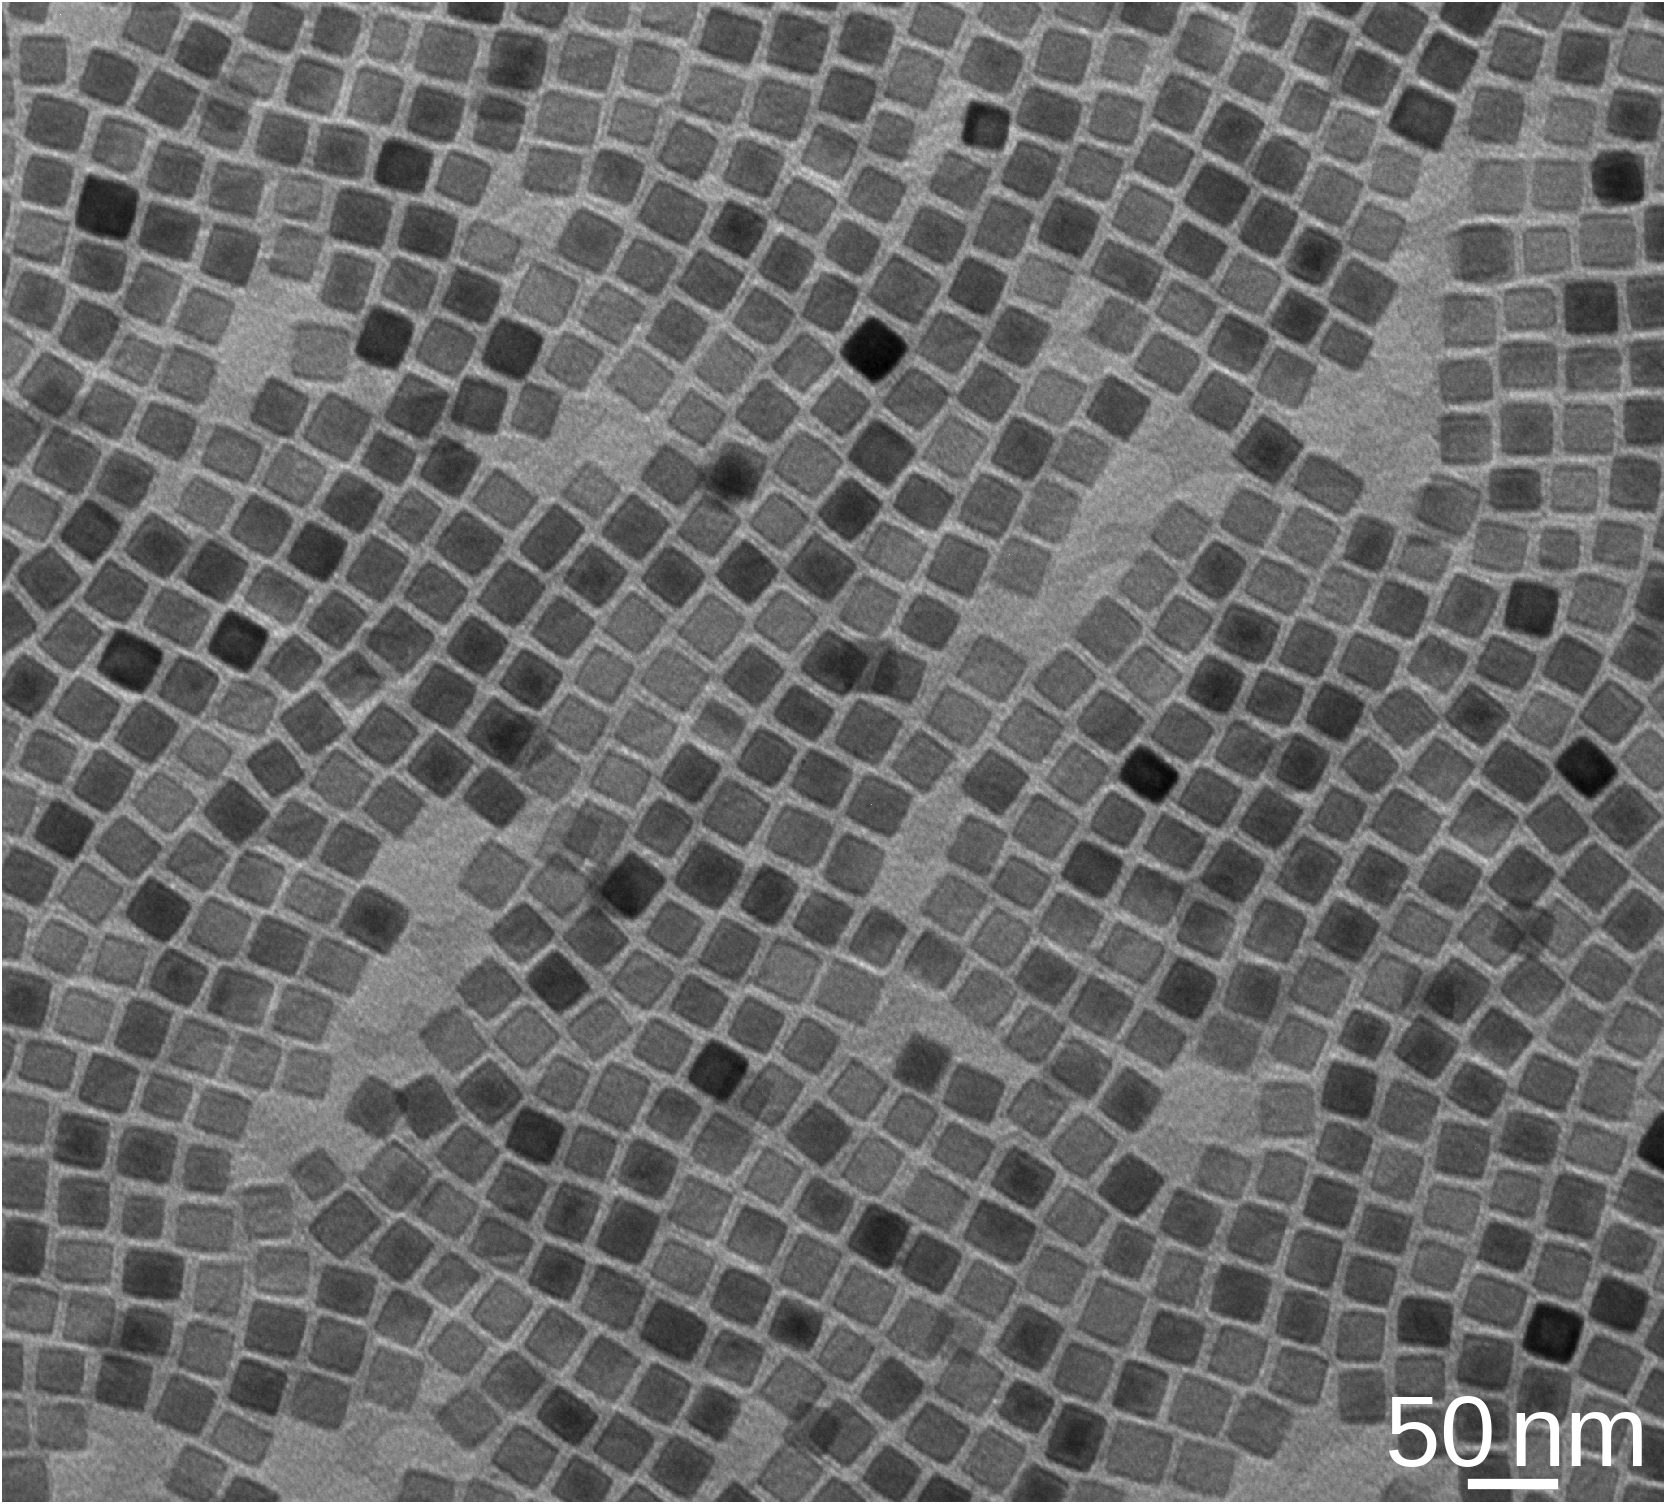
\includegraphics{monolayers_TEM_Ol_CoFe_C}
      \hspace{0.3 cm}
      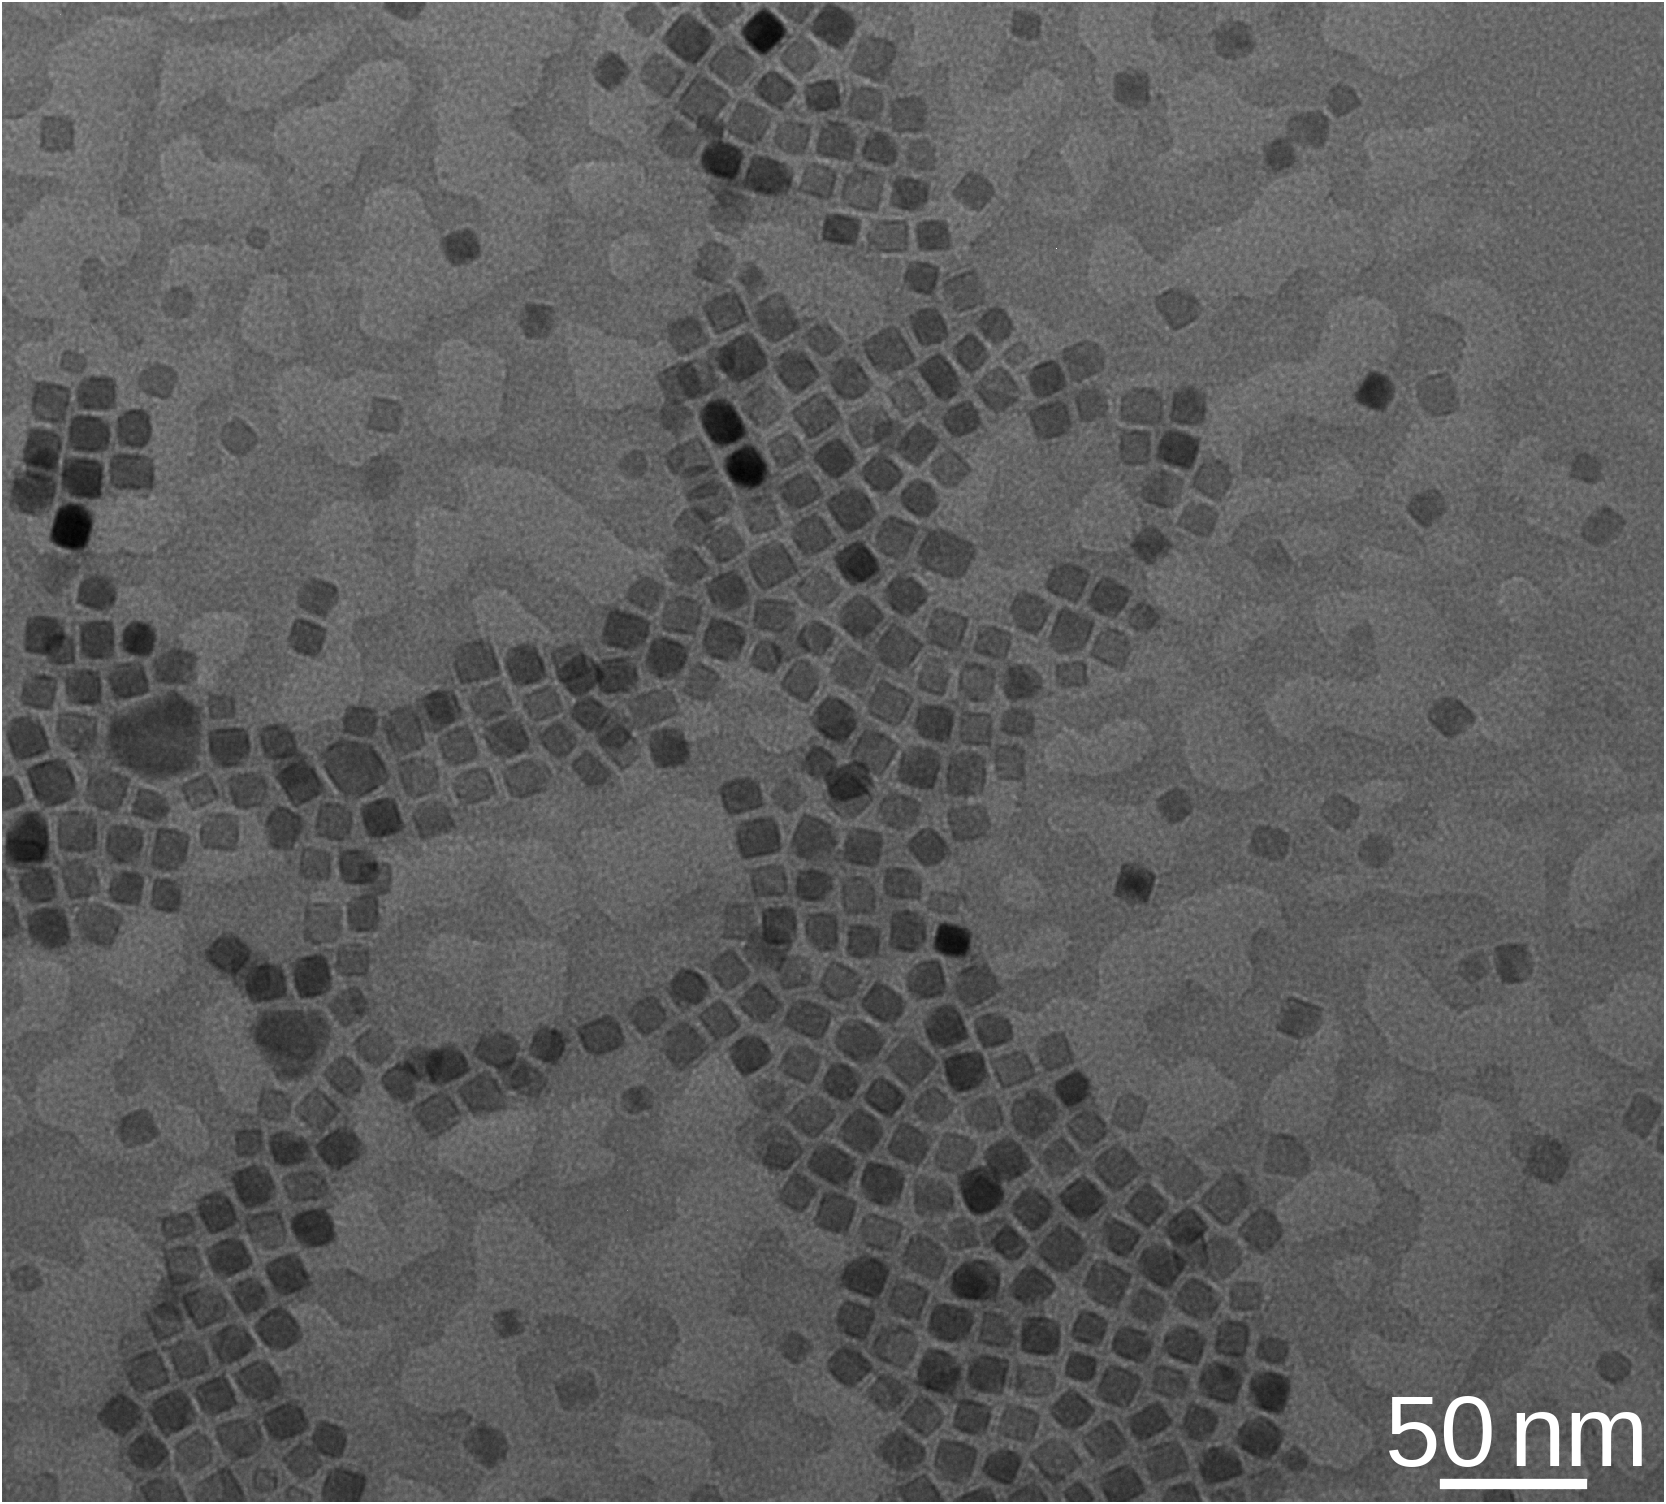
\includegraphics{monolayers_TEM_Ac_CoFe_C}
      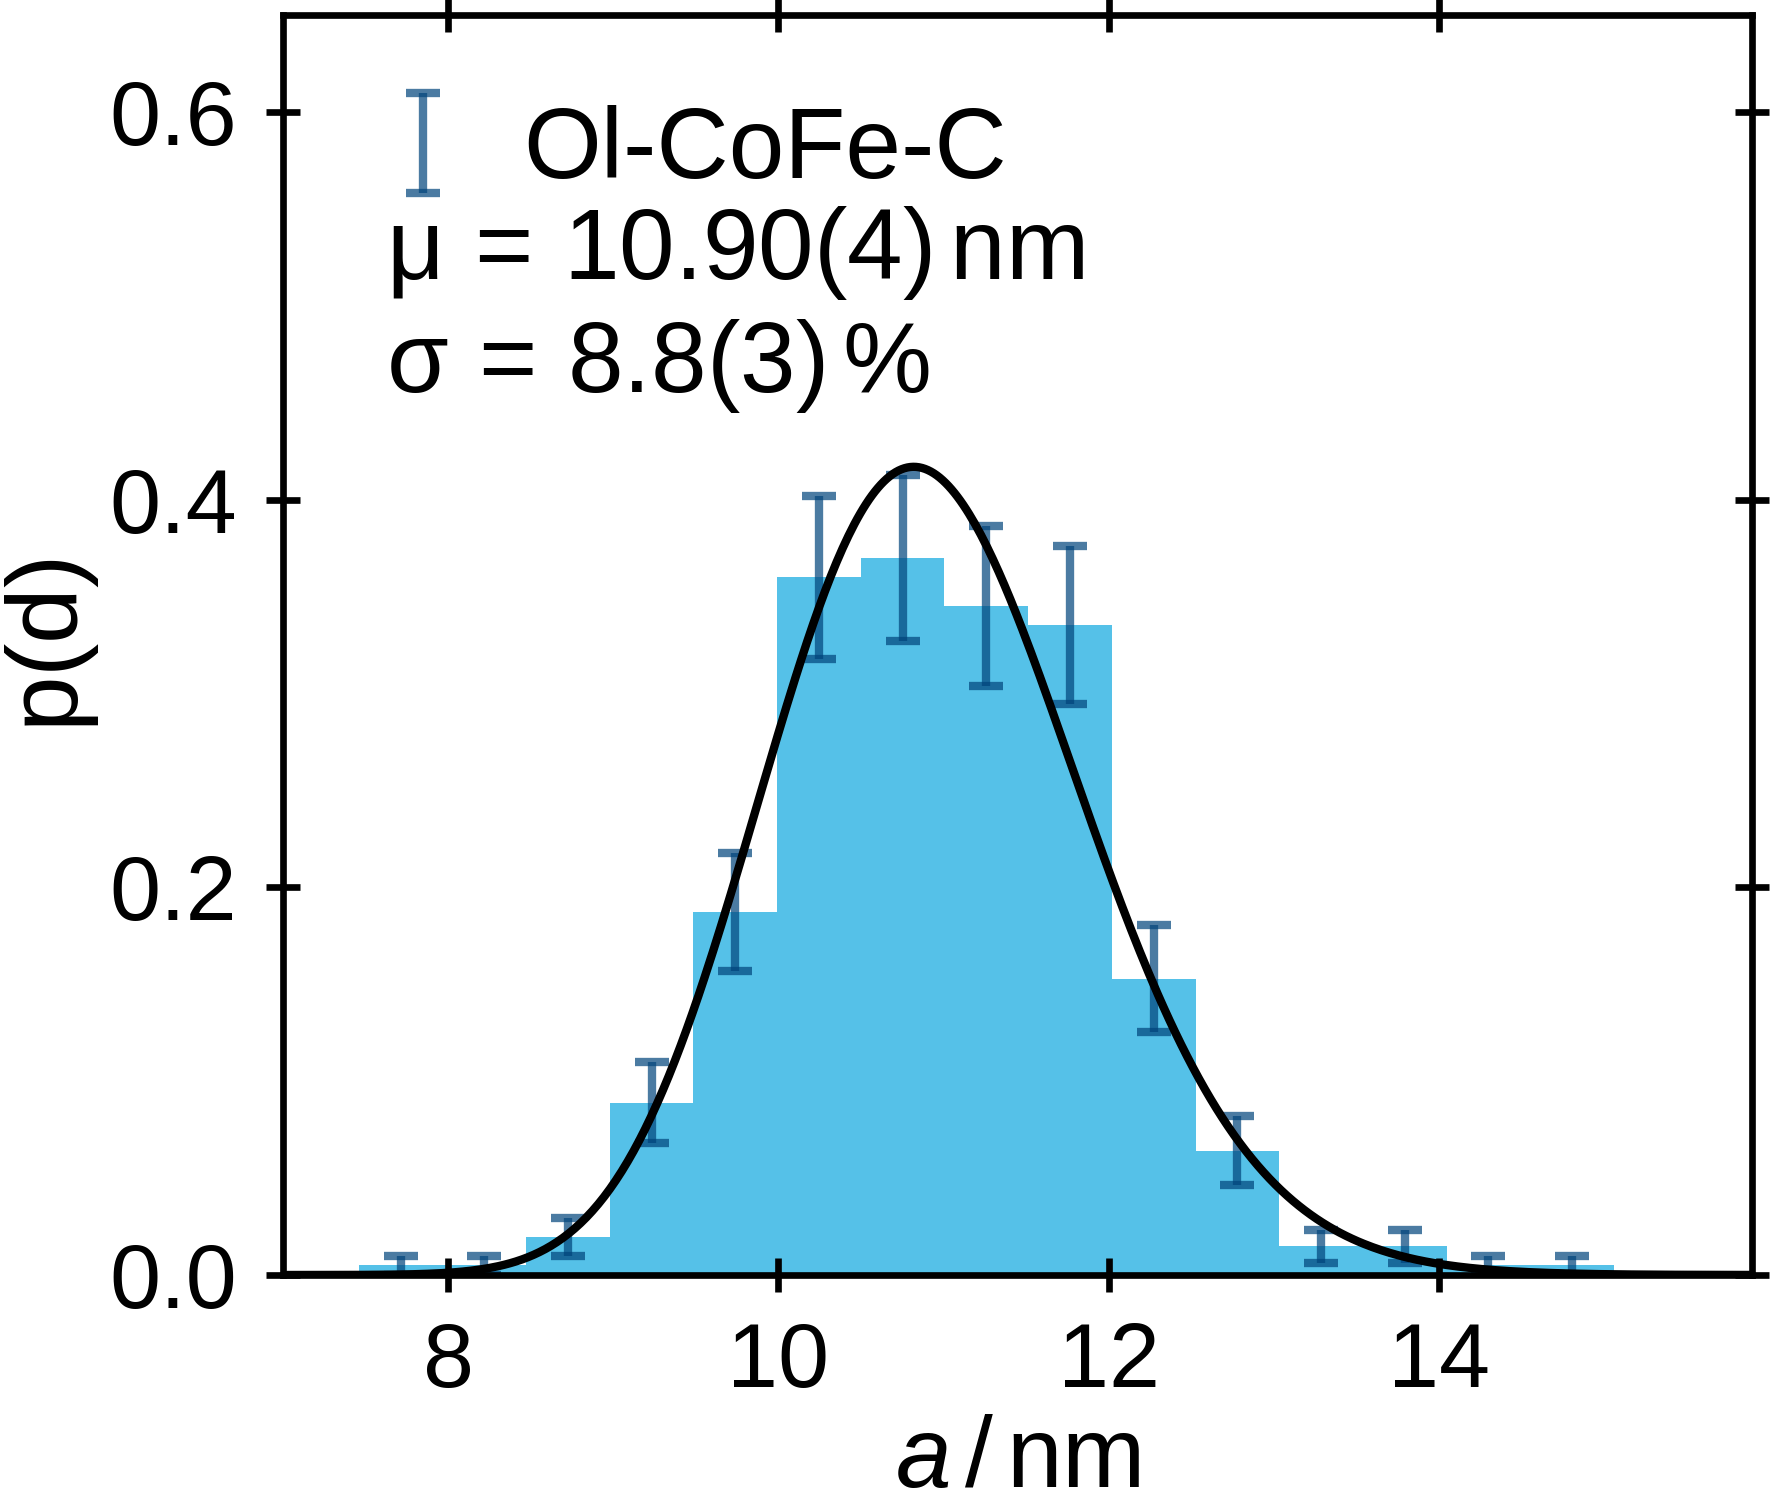
\includegraphics{monolayers_TEM_Ol_CoFe_C_sizeDist}
      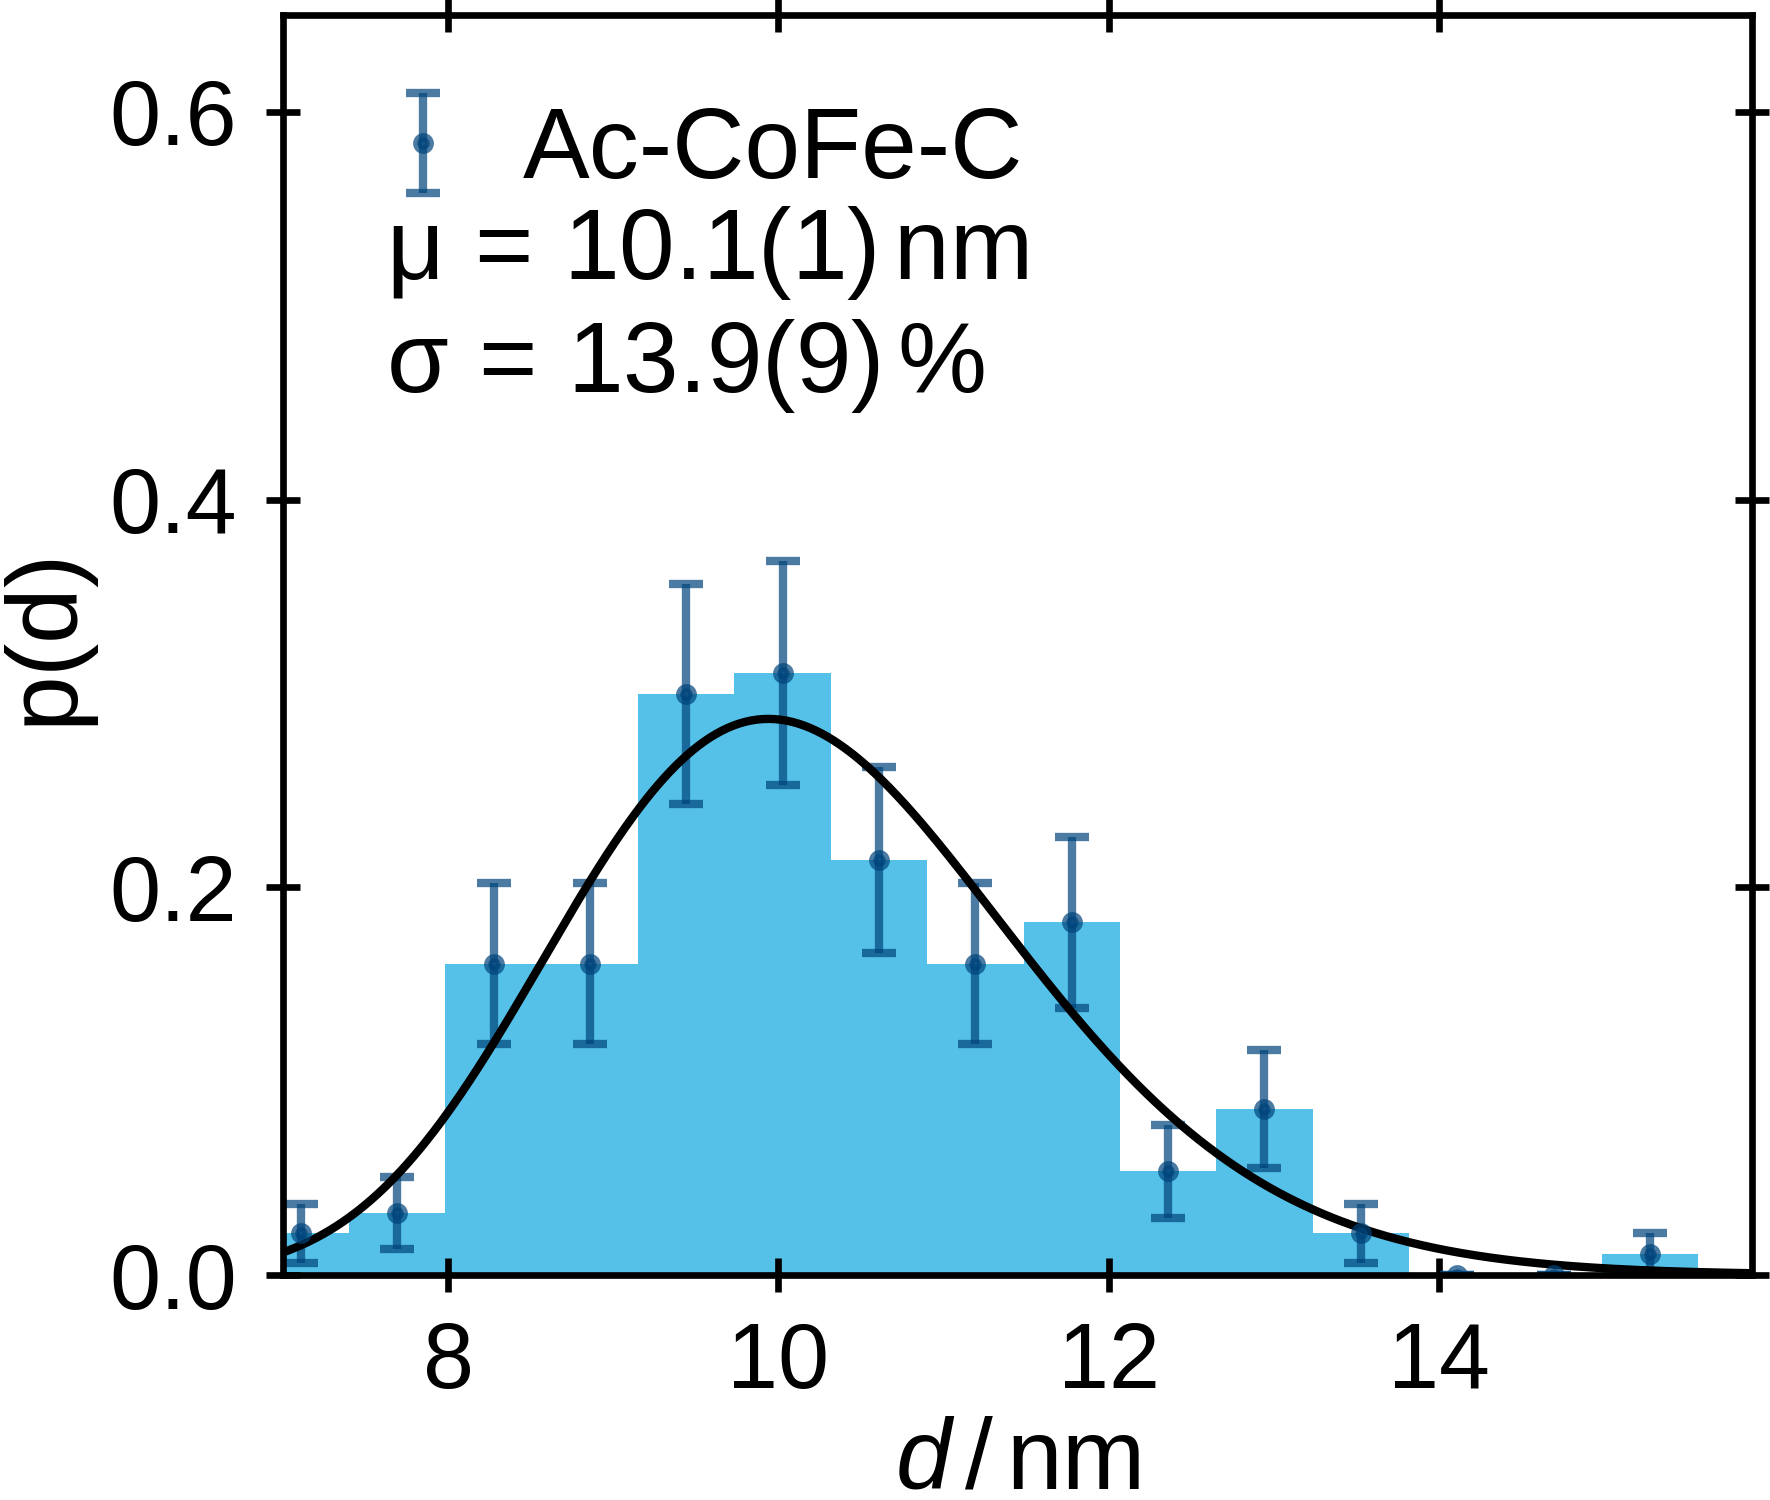
\includegraphics{monolayers_TEM_Ac_CoFe_C_sizeDist}
      \caption{\label{fig:monolayers:nanoparticle:tem}Bright field TEM micrographs of cobalt ferrite nanocubes synthesized from oleates (upper left) and acetylacetonates (upper right) and the edge length size distribution evaluated from the images below respectively.}
    \end{figure}

    A macroscopic area of the samples is quantitatively evaluated to determine the average nuclear and magnetic structure of the diluted nanoparticles in dispersion using small-angle X-ray and (polarized) neutron scattering in \reffig{fig:monolayers:nanoparticle:sas:AcOlCoFeC}.
    For the SAXS measurement, the samples were diluted in n-hexane and measured at the GALAXI instrument in the \textsc{Forschungszentrum J\"ulich}, which is described in \refapp{ch:appendix:lss:galaxi}.
    The small-angle neutron scattering data was measured using the D22 and D33 instrument at the Institut Laue-Langevin, which are described in \refapp{ch:appendix:lss:d22} and \refapp{ch:appendix:lss:d33} respectively.
    For the neutron scattering experiment, the sample was dried and redispersed in deuterated toluene ($\mathrm{toluene-d_8}$) to reduce the incoherent scattering coming from hydrogen atoms.
    The comparison between the Ol-CoFe-C and Ac-CoFe-C small-angle scattering data shows on a qualitative level that the nanocubes synthesized following the oleate route have a smaller size distribution and higher homogeneous sample quality as more oscillations are visible with more pronounced minima, confirming the result observed from TEM.
    However, it also shows that Ol-CoFe-C is only weakly magnetic whereas the particles in Ac-CoFe-C have a stronger magnetic moment, which is visible in the greater splitting of $I(+)$ and $I(-)$ in SANSPOL.

    \begin{figure}[tb]
      \centering
      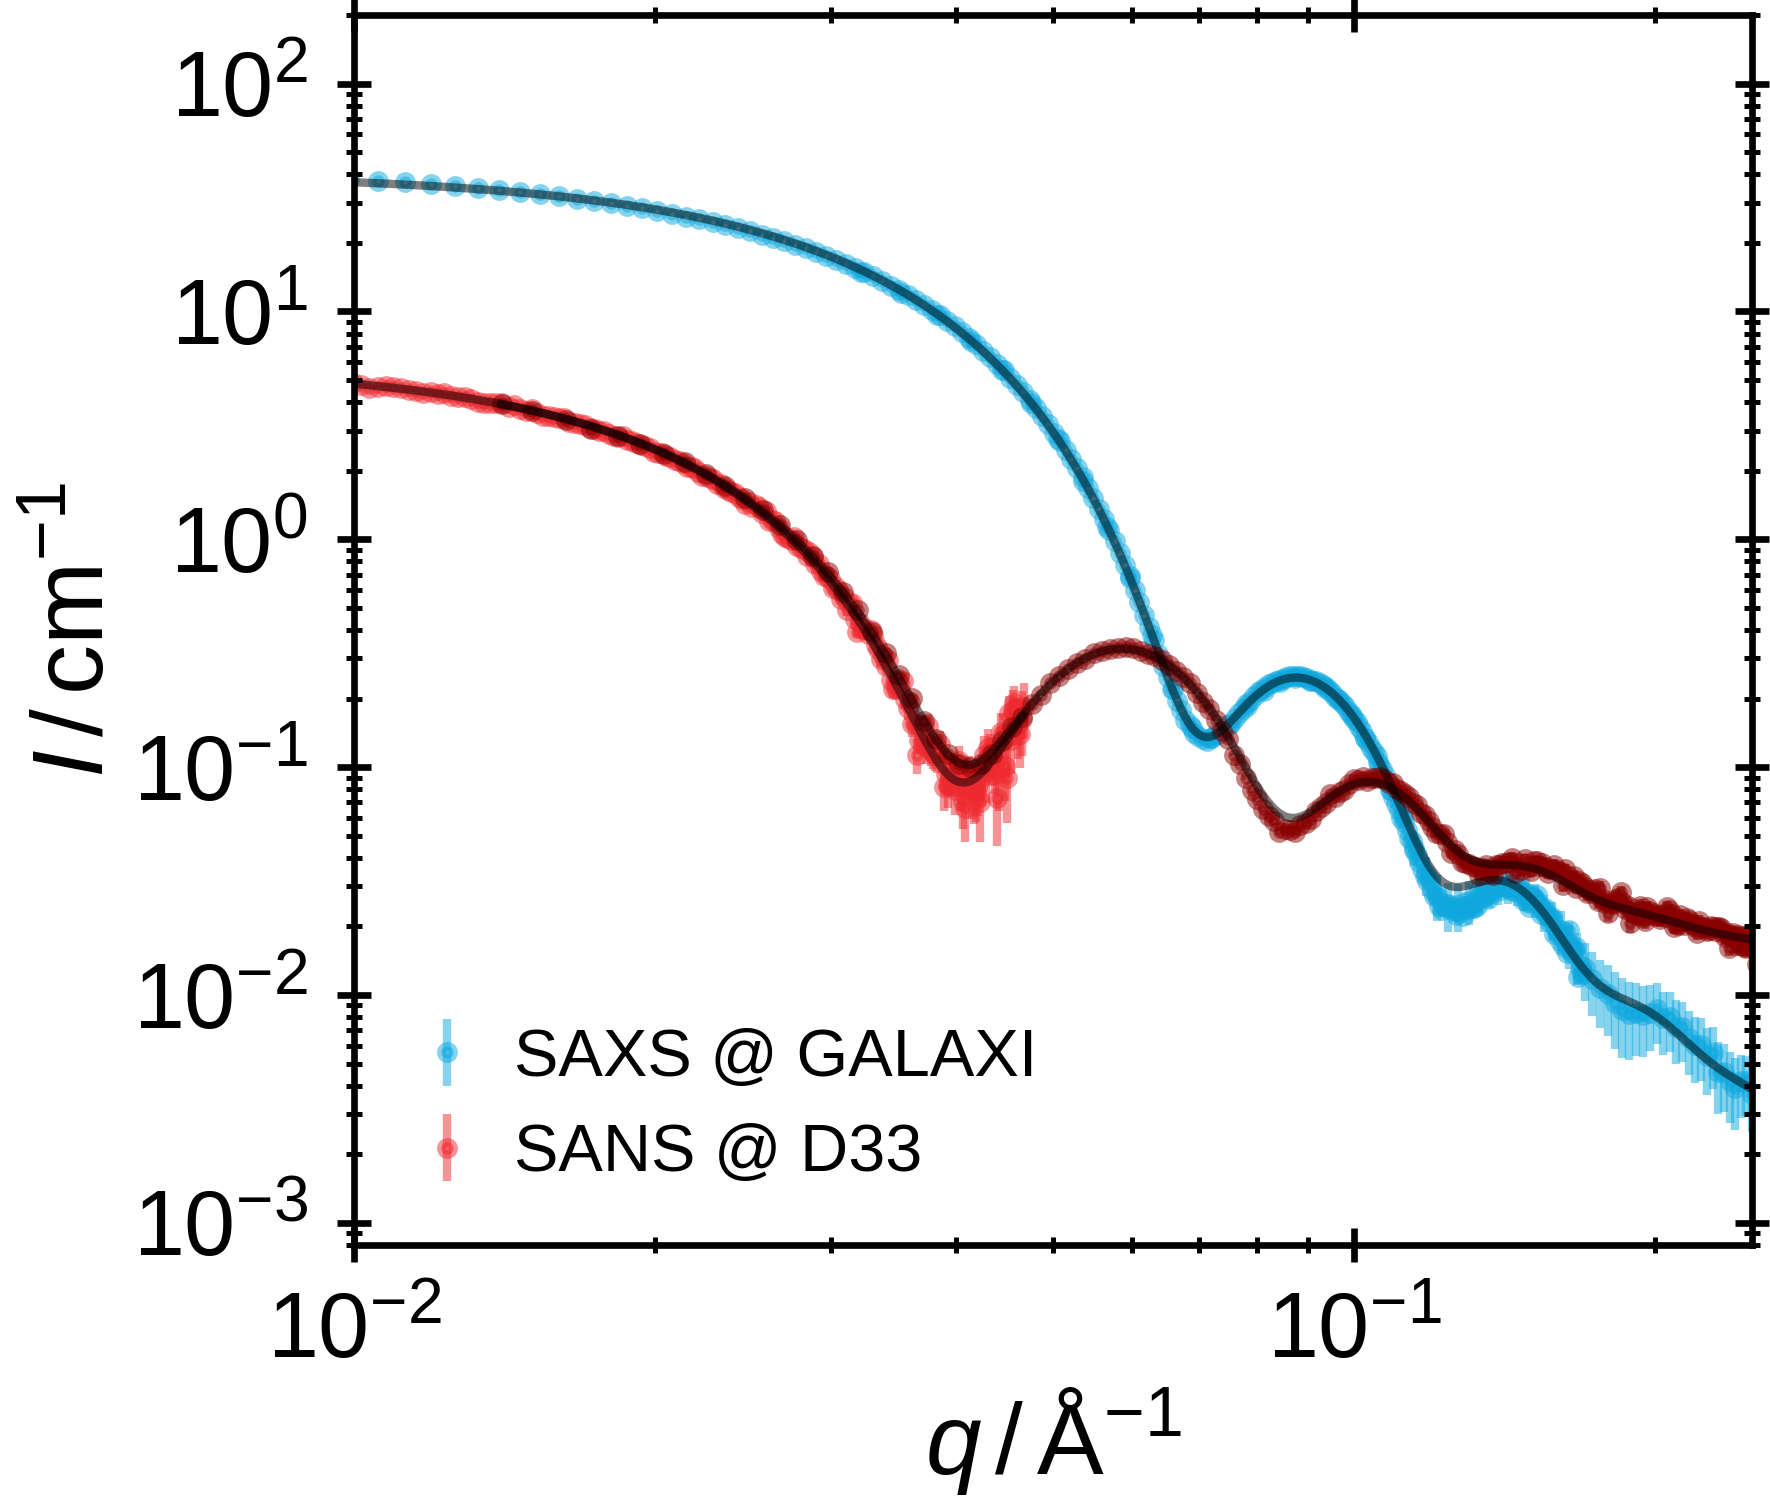
\includegraphics{monolayers_SAS_Ol_CoFe_C_SASFit}
      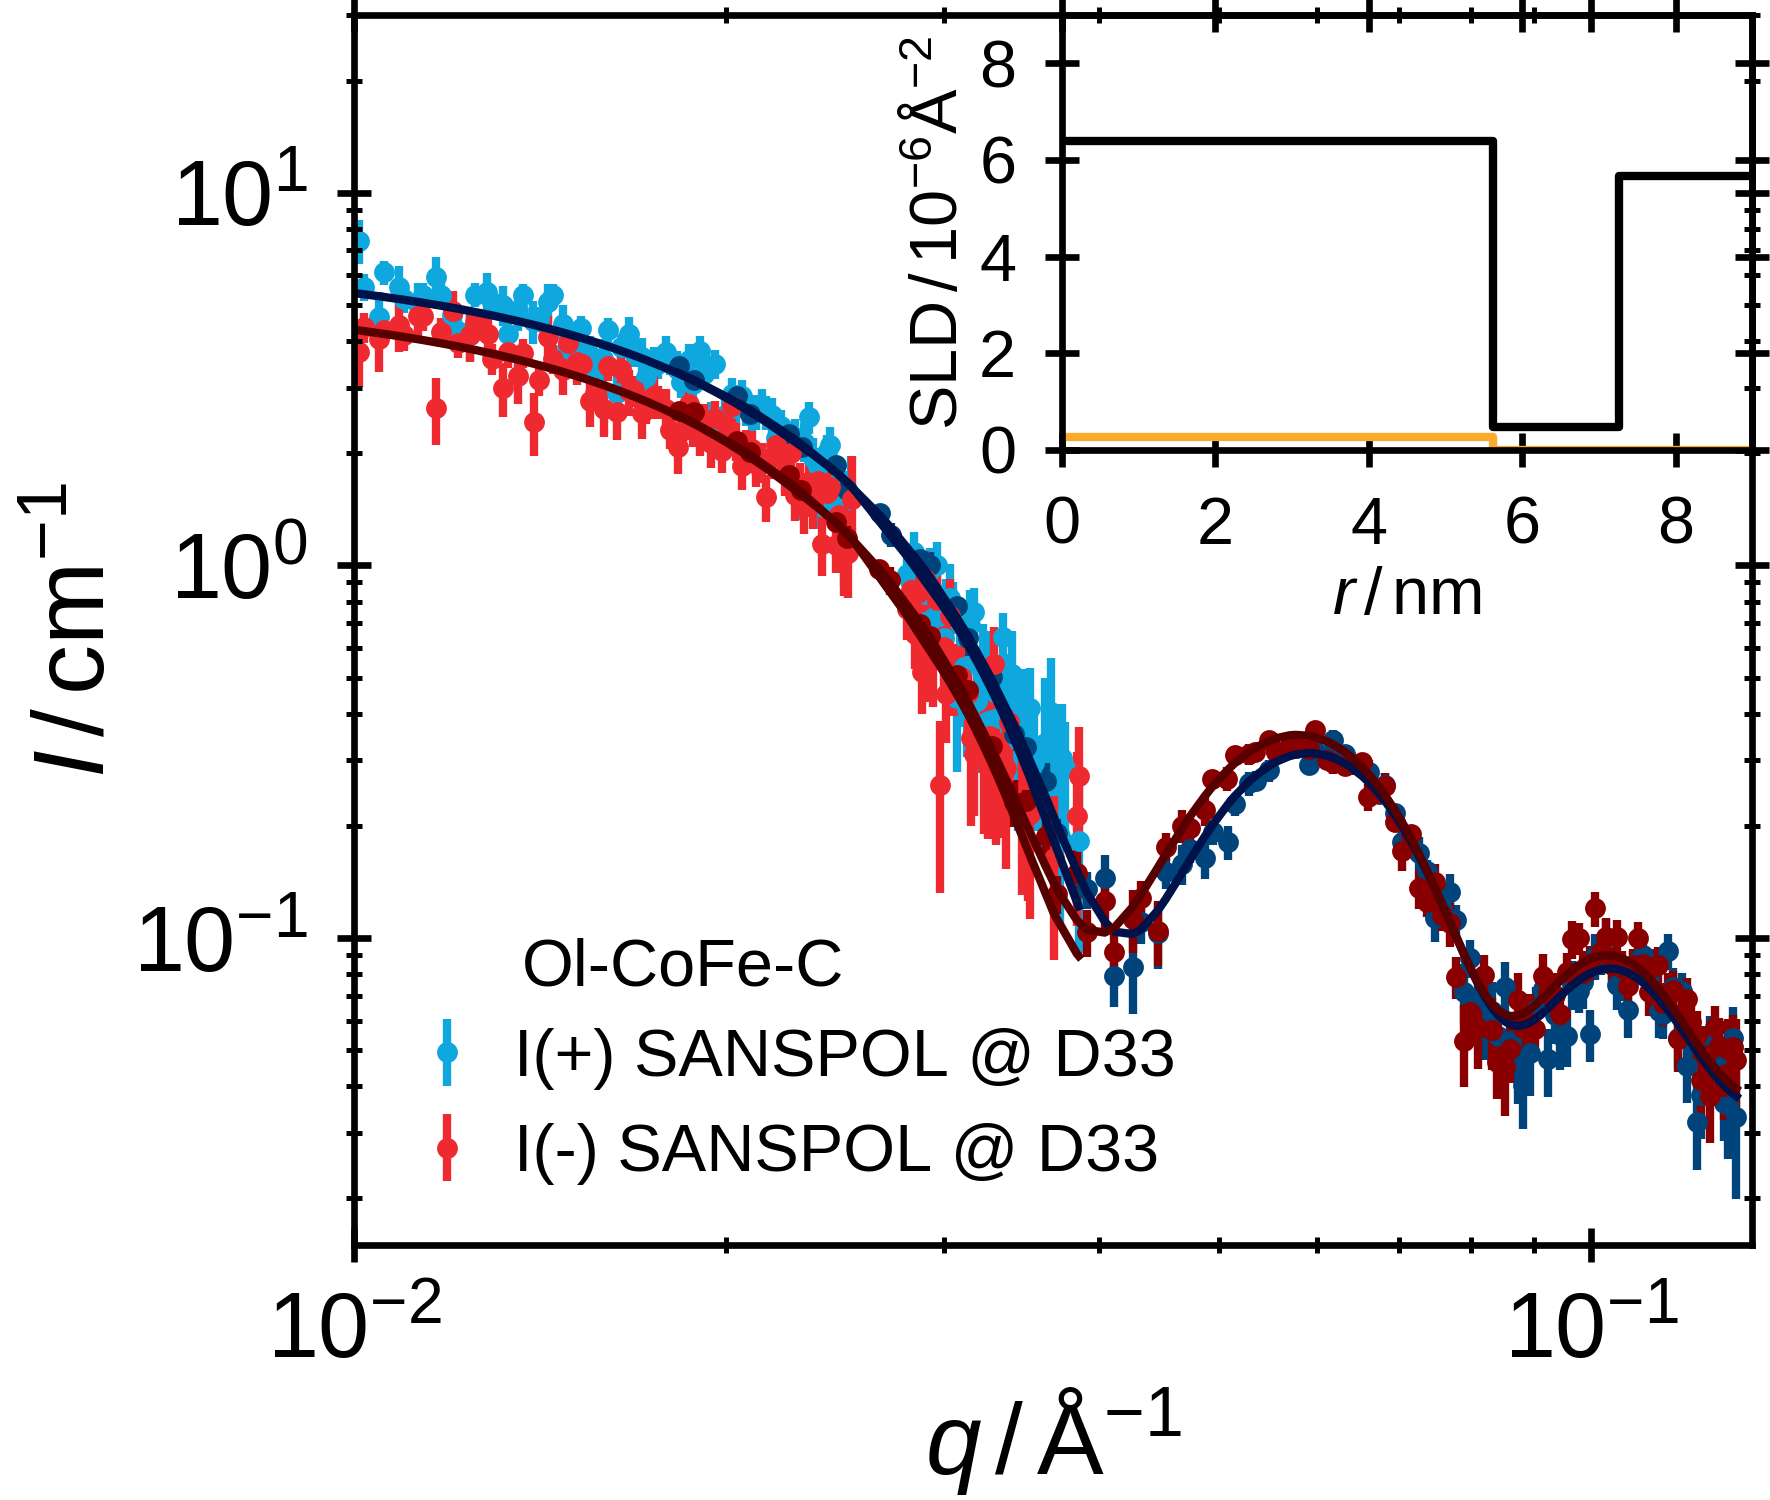
\includegraphics{monolayers_SAS_Ol_CoFe_C_SANSPOLFit}
      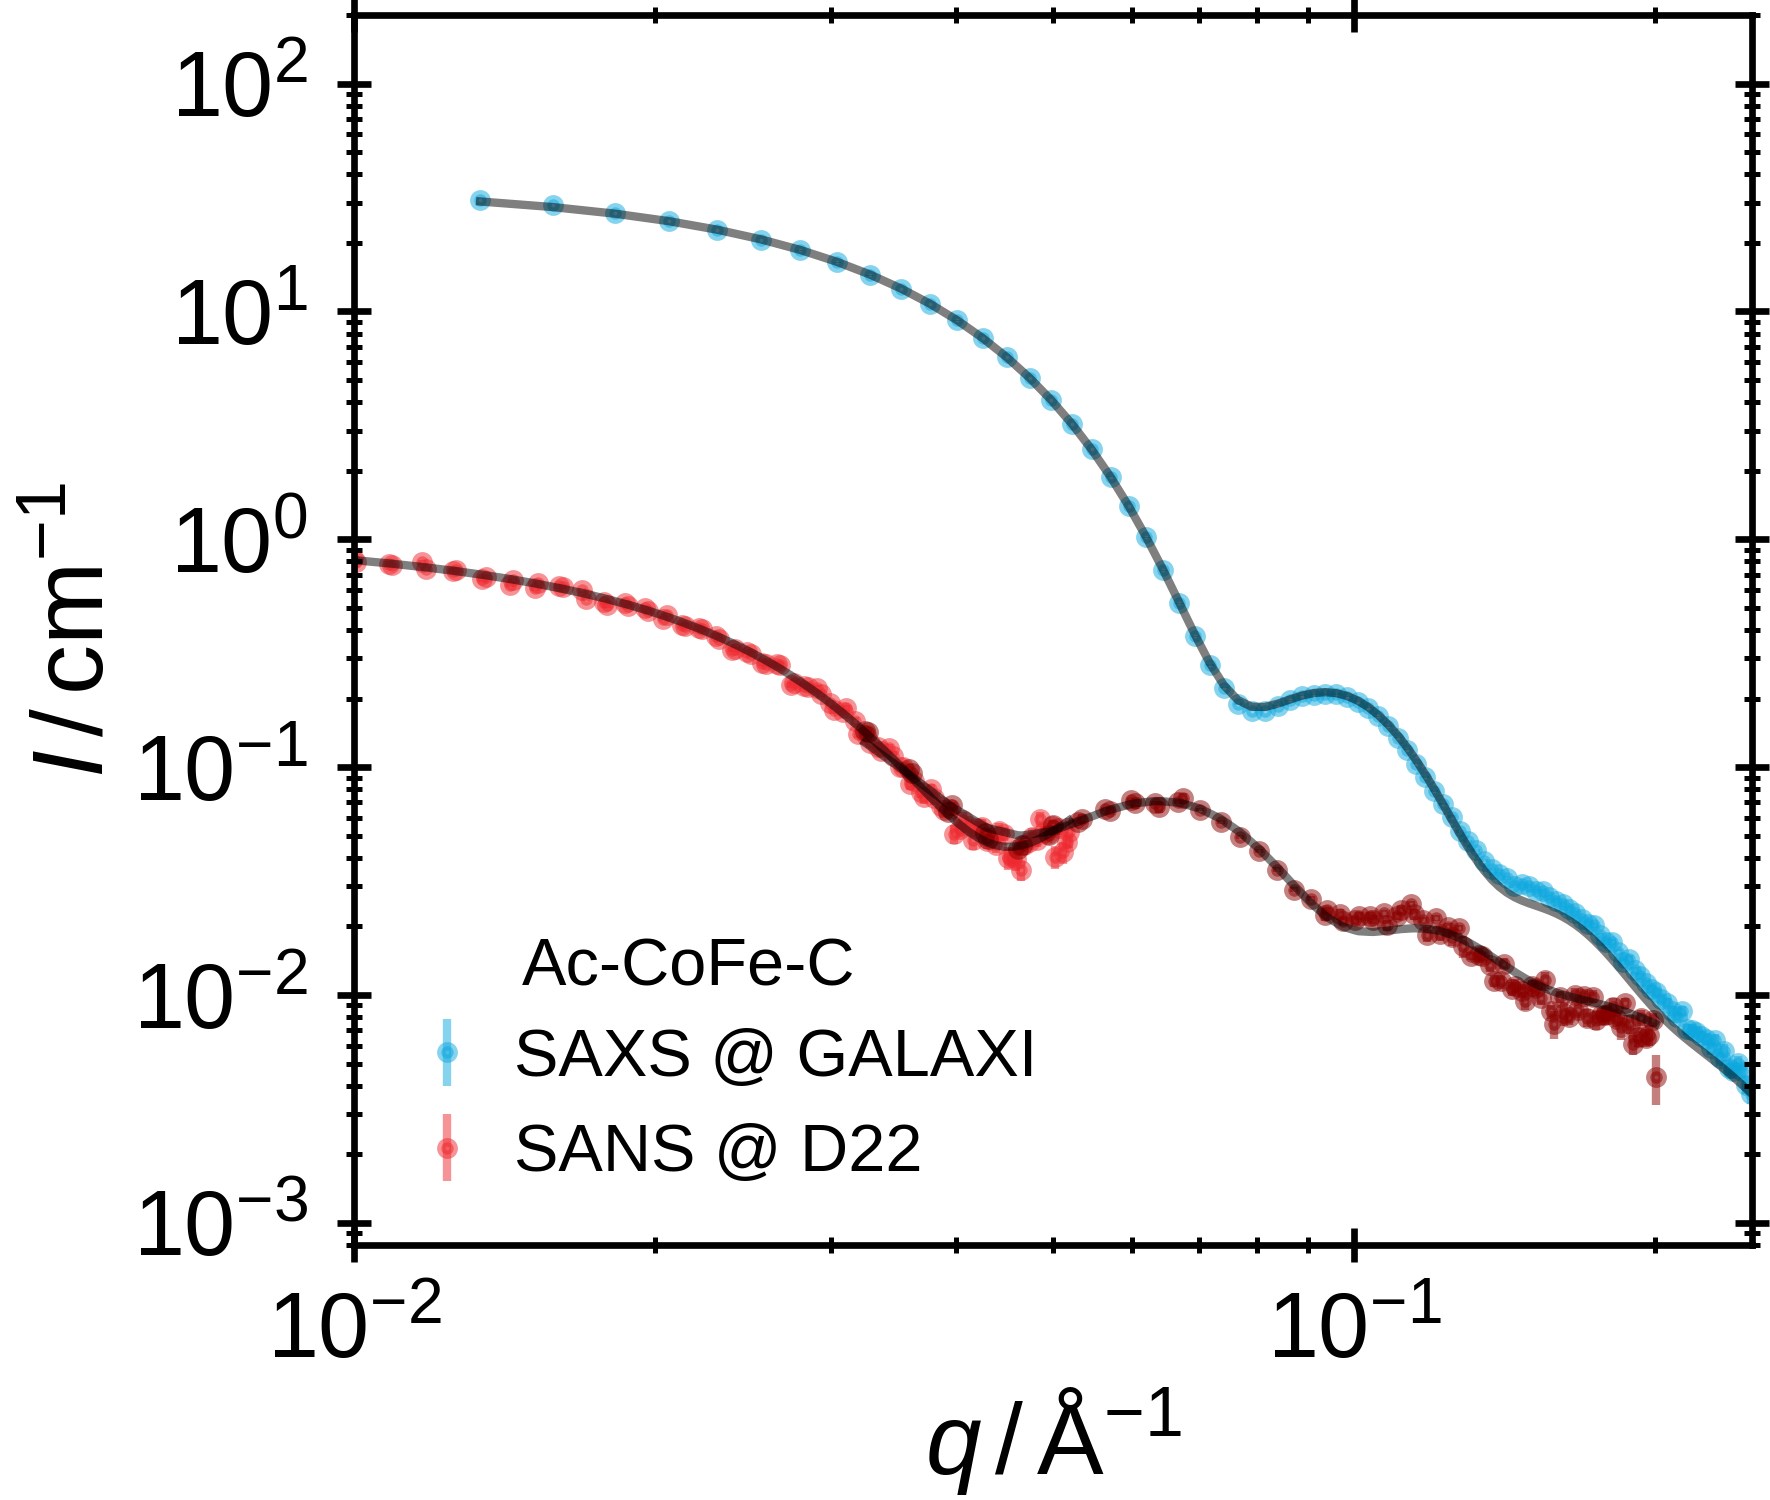
\includegraphics{monolayers_SAS_Ac_CoFe_C_SASFit}
      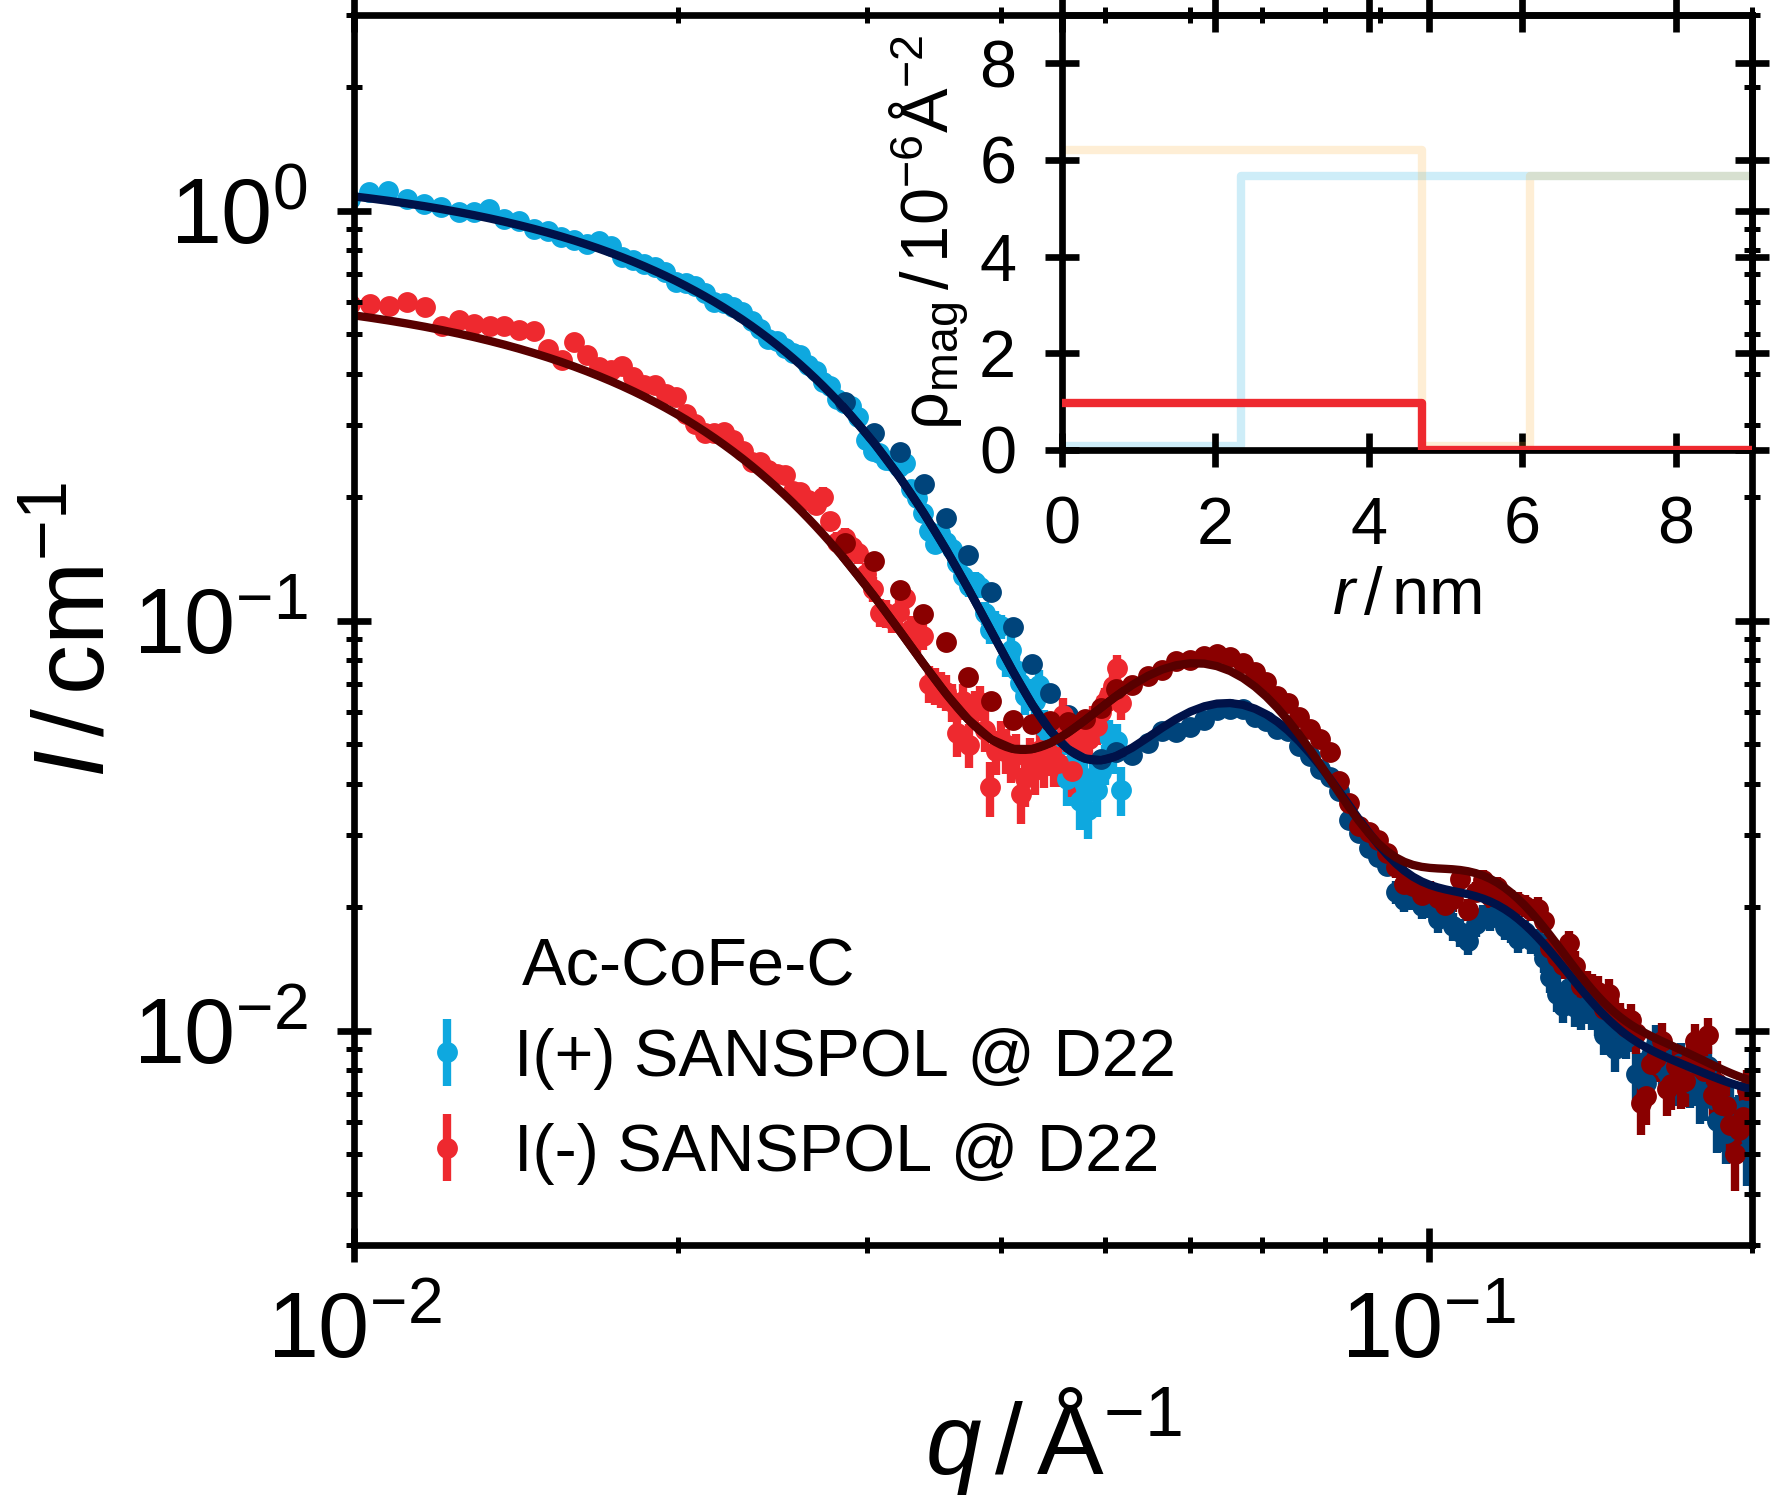
\includegraphics{monolayers_SAS_Ac_CoFe_C_SANSPOLFit}
      \caption{\label{fig:monolayers:nanoparticle:sas:AcOlCoFeC}SAXS and SANS measurement of Ol-CoFe-C (upper left) and Ac-CoFe-C (lower left), as well as SANSPOL at $1.2 \unit{T}$ respectively (right). The data is fit to a superball model.}
    \end{figure}

    To evaluate the data quantitatively, the data of both samples is used to fit the parameters of a superball model.
    Briefly, a superball is a mathematical shape that can be used to describe rounded cubes and it's volume is defined by
    \begin{align}
      x^{2p} + y^{2p} + z^{2p} < R^{2p},
    \end{align}
    where $R$ is the radius of the superball and $p$ describes whether the body is closer to a sphere or a cube.
    For $p\eq 1$ the superball is equivalent to the definition of a sphere and for $p \rightarrow \infty$ the superball converges to a cube with edge length $a \eq 2R$.
    The full description and derivation of the superball properties and formfactor is described in \refapp{ch:appendix:numericalMethods:superballFormfactor}.
    To account for the oleic acid surfactant of the nanoparticles, the superball volume is assumed to have a core-shell structure, where the shell is variable in scattering length density and thickness.
    The fitted model is shown in \reffig{fig:monolayers:nanoparticle:sas:AcOlCoFeC} and the important parameter of interest are given in \reftab{tab:monolayers:nanoparticle:sas} for the following discussion, whereas the full set of model parameters is listed in \refapp{ch:appendix:modelparameters:monolayers:sas_olac_cofe_c}.
    \begin{table}[ht]
      \centering
      \caption{\label{tab:monolayers:nanoparticle:sas}Relevant parameters of the superball fit of the small-angle scattering data of the presented nanocubes, the complete set used to describe the models are found in \refapp{ch:appendix:modelparameters:monolayers:sas_olac_cofe_c}.}
      \begin{tabular}{ c | l | l }
          & Ol-CoFe-C & Ac-CoFe-C \\
        \hline
        $R$
          & $5.62(2) \unit{nm}$
          & $4.69(1) \unit{nm}$\\
        $\sigma_R$
          & $9.27(8) \,\%$
          & $11.9(1) \,\%$\\
        $D$
          & $1.63(1) \unit{nm}$
          & $1.16(4) \unit{nm}$\\
        $p$
          & $1.54(3) \unit{nm}$
          & $2.66(9) \unit{nm}$\\
        $\rho_\mathrm{mag}^\mathrm{sans}$
          & $0.268(8) \cdot 10^{-6} \angstrom^{-2}$
          & $0.423(7) \cdot 10^{-6} \angstrom^{-2}$\\
        \hline
        $V_p$
          & $1030(10) \unit{nm^3}$
          & $726(5) \unit{nm}$\\
        $M^\mathrm{sans}$
          & $92(3) \unit{kAm^{-1}}$
          & $145(2) \unit{kAm^{-1}}$\\
        \hline
      \end{tabular}
    \end{table}
    The superball model result confirms the qualitative observation that the Ol-CoFe-C nanoparticles have a smaller size distribution than the Ac-CoFe-C cubes.
    Where the specimen size used to determine size and size distributions in TEM leave the option for a biased result due to possibly missed counting fractions of the dispersion by only measuring a small selected amount of nanoparticles, the large number of particles scanned in the small-angle scattering experiments reveals without bias the average particle size and variation.
    Furthermore, the model gives that on average Ol-CoFe-C has a higher degree of roundness on the corners, visible from the smaller $p$ parameter in comparison to Ac-CoFe-C.
    To see this in imaging experiments, high resolution transmission electron microscopy (HR-TEM) experiments are necessary.
    A study comparing the effectiveness of the superball model in comparison to HR-TEM can be found in \refapp{app:structureCoFe2O4Nanocubes} for three particle batches synthesized similar to Ac-CoFe-C (with a lower heating rate and varied cobalt content, but otherwise same synthesis parameters).

    \begin{figure}[tb]
      \centering
      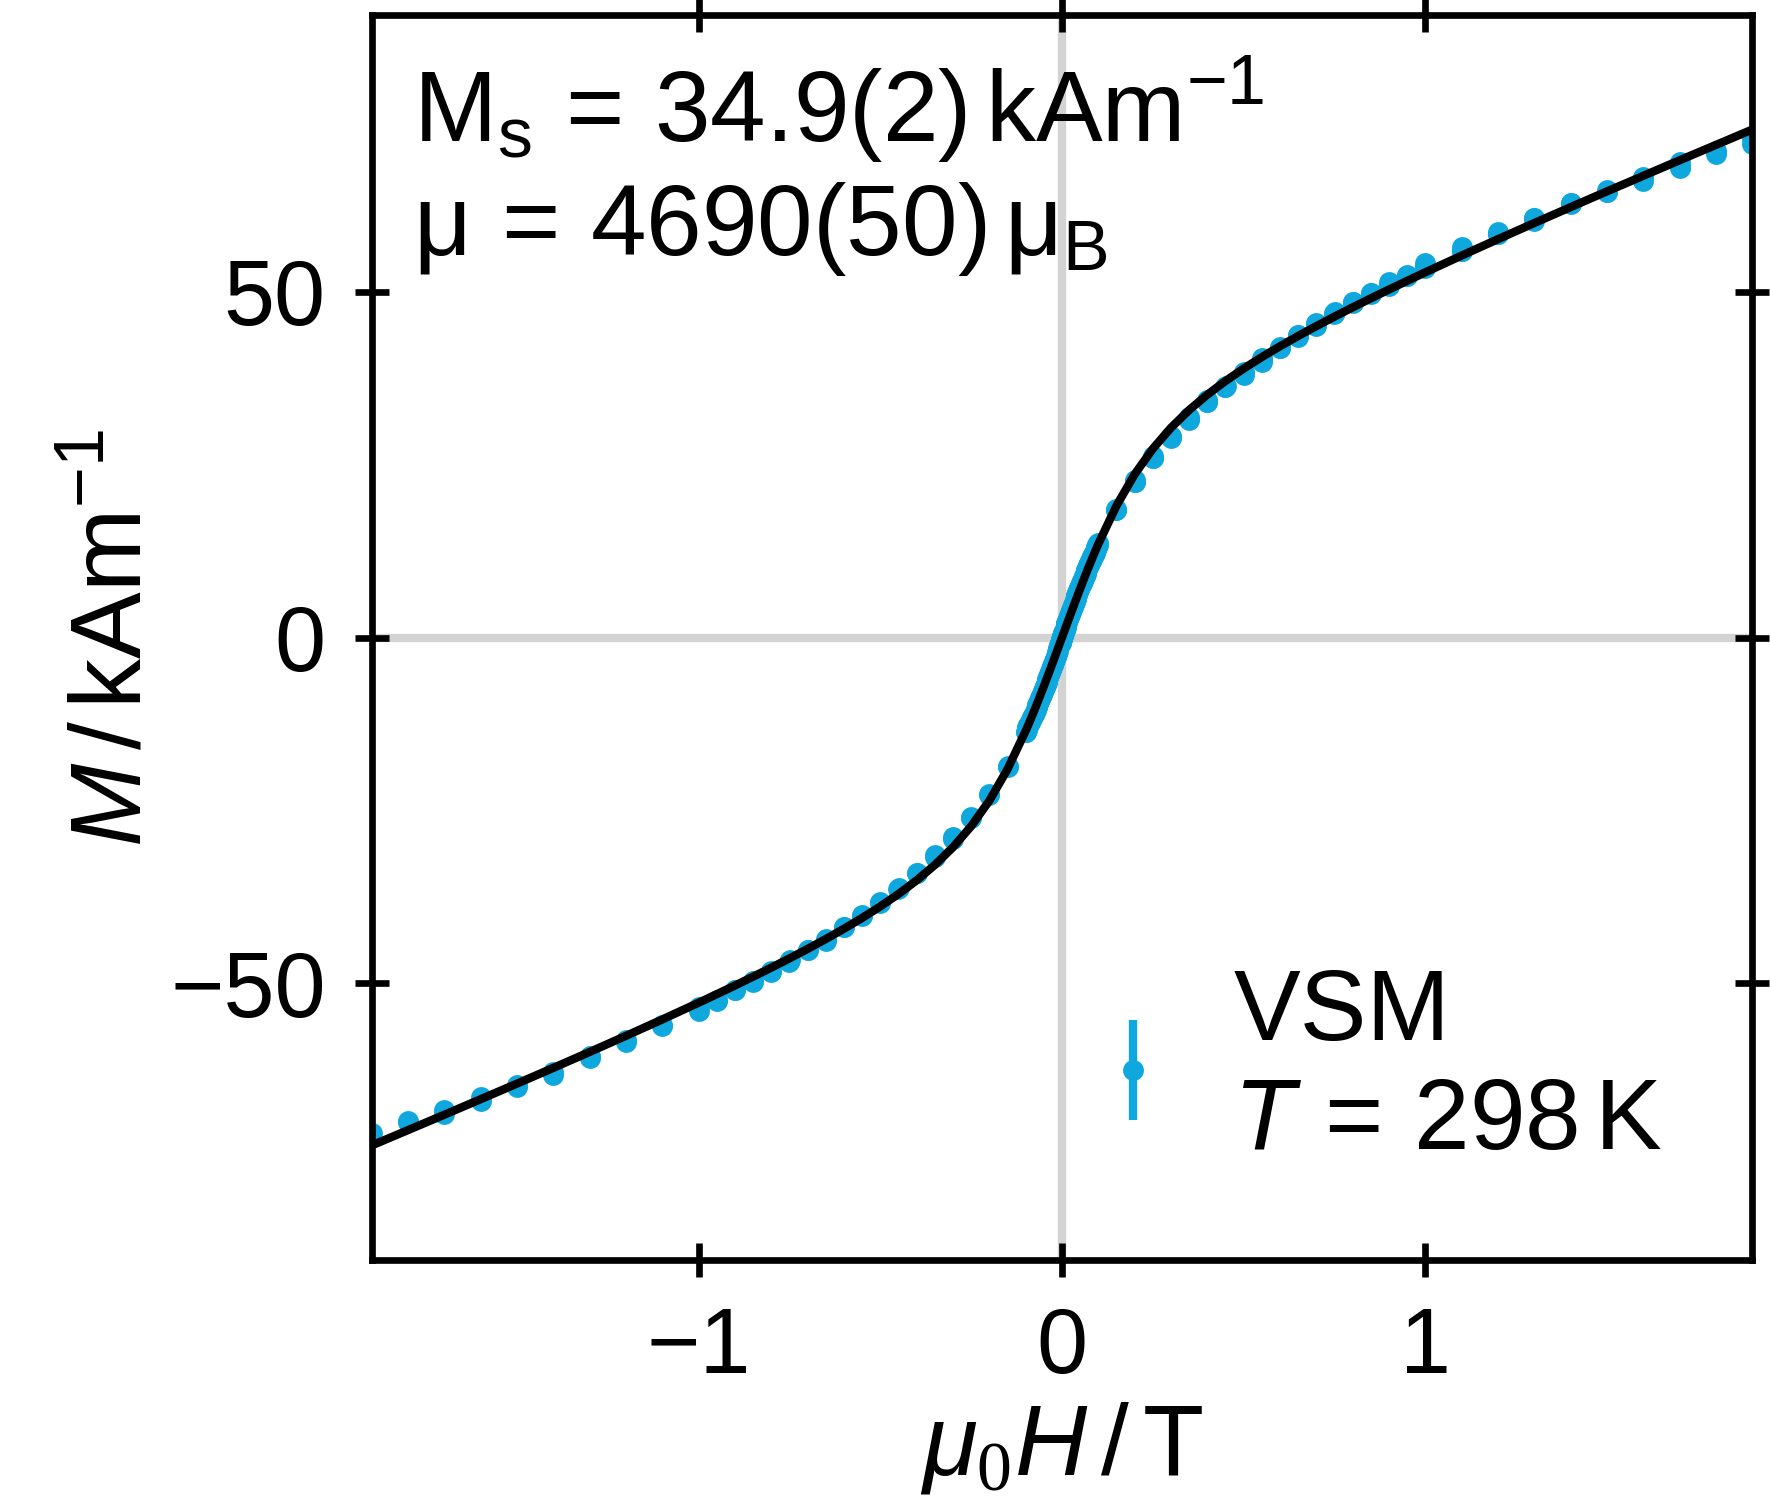
\includegraphics{monolayer_VSM_Ol_CoFe_C}
      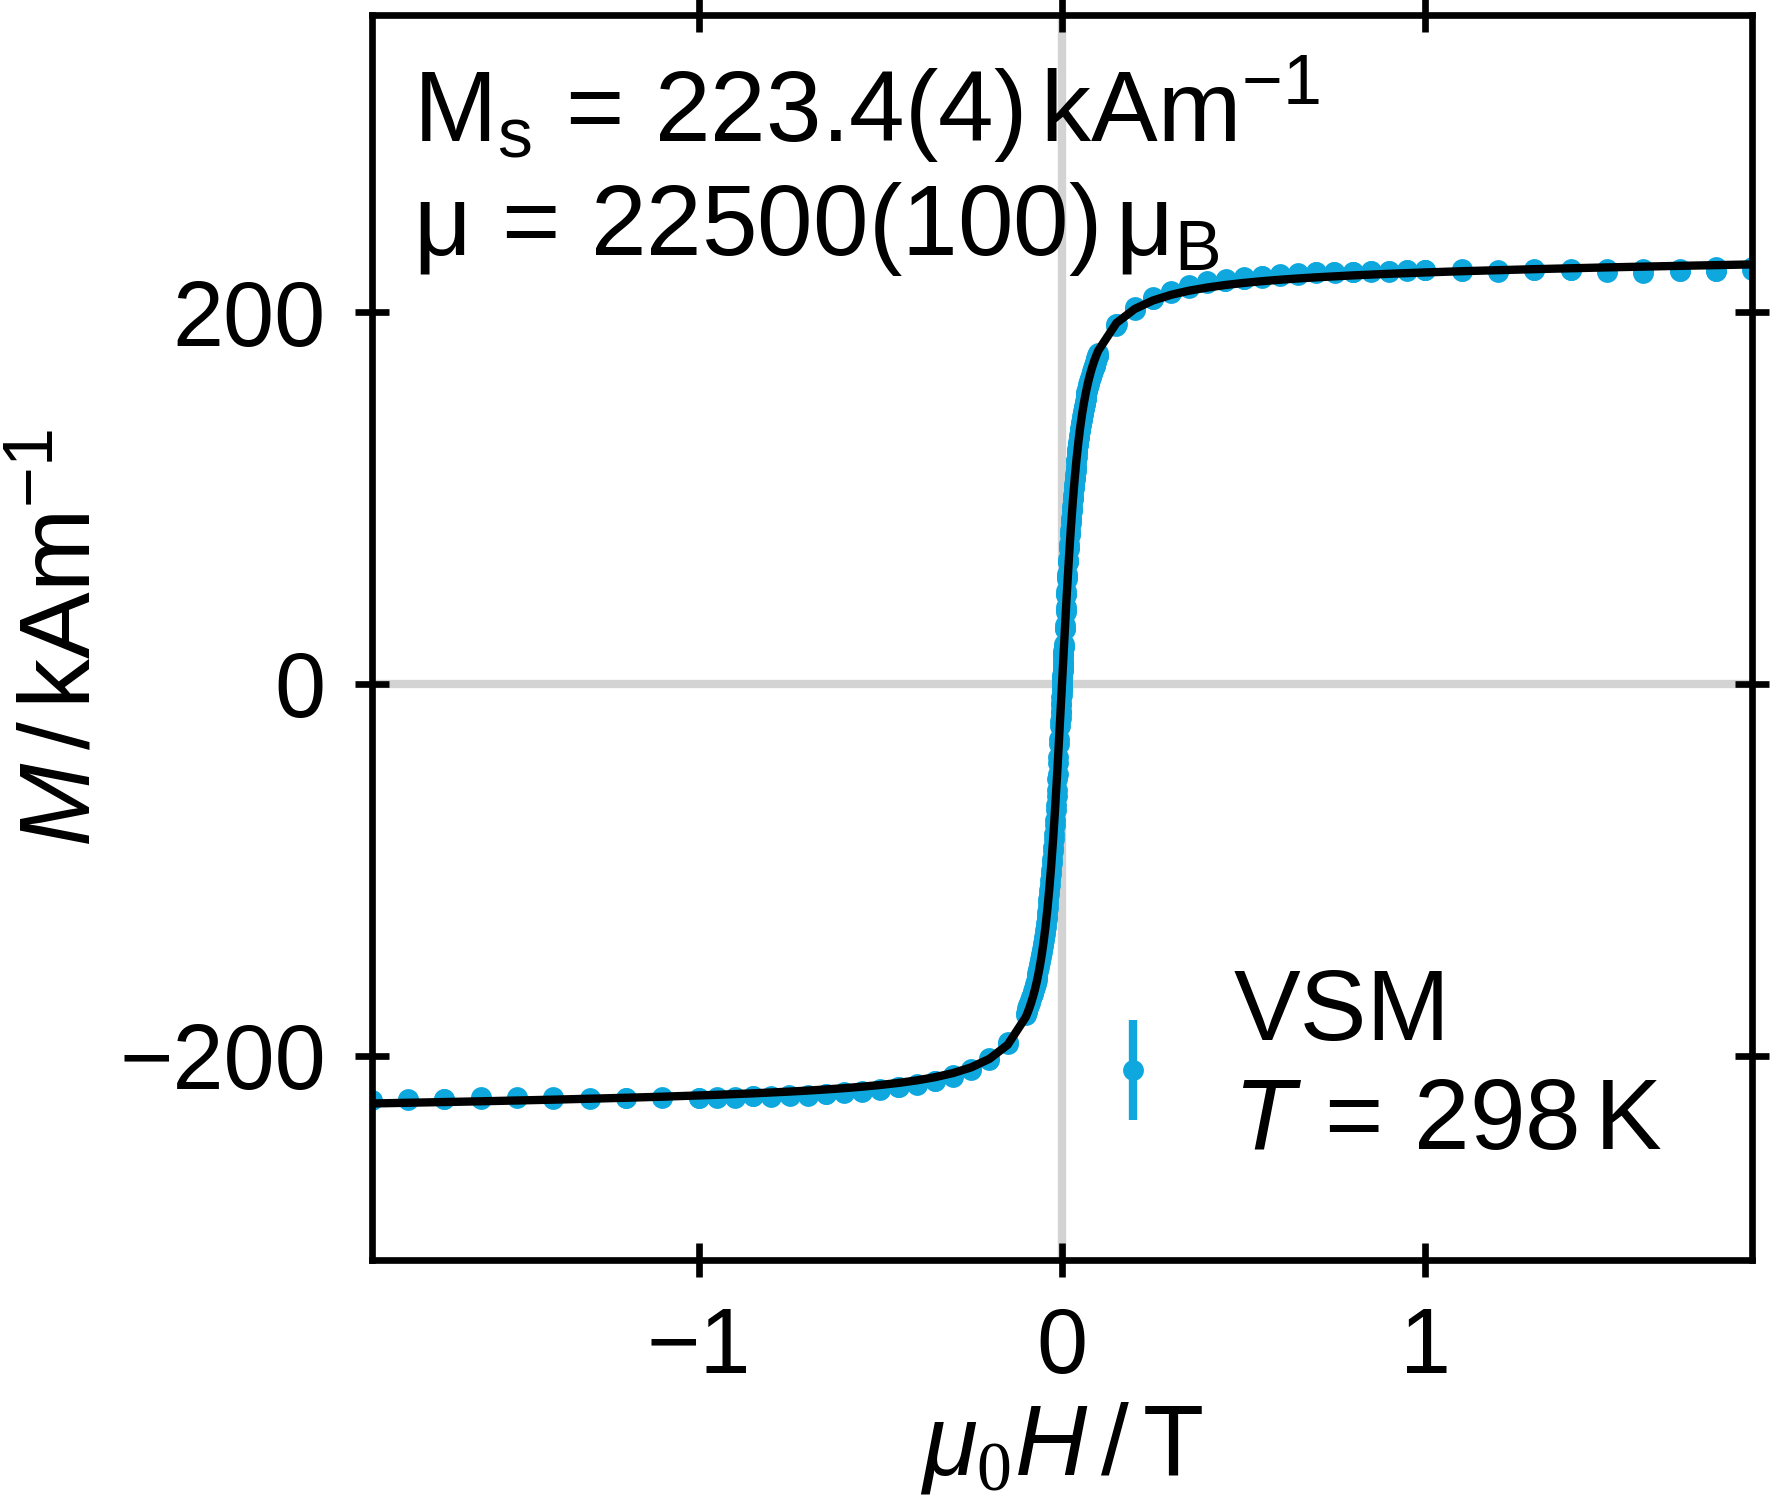
\includegraphics{monolayer_VSM_Ac_CoFe_C}
      \caption{\label{fig:monolayers:nanoparticle:vsm}Room-temperature hysteresis of Ol-CoFe-C (upper left) and Ac-CoFe-C (lower left) dried on a substrate measured using a vibrating sample magnetometer and fitted with a Langevin curve.}
    \end{figure}
    The surfactant shell thickness are in the range of $1 - 2 \unit{nm}$, which is expected for oleic acid chains.
    As the chains mix with the solvent on the way out, it is expected that the average scattering length density of the shell is not exactly that of bulk oleic acid ($7.8 \cdot 10^{-8} \angstrom^{-2}$), but a mixture with the solvent SLD, which correlates with the model thickness and might explain the reduced value in Ac-CoFe-C.
    The exact thickness, density and shape of the shell is not of detailed interest for the study of the magnetic properties of the nanocubes and therefore in the scope of this work this rough estimate of the shell is good enough for the discussion.

    % SANSPOL <-> VSM at 300K
    The magnetic scattering length density is determined from the SANSPOL data, which is used to determine the magnetization of the nanoparticle using \refeq{eq:looselyPackedNP:nanoparticles:SLDtoMagnetization} to $92(3) \unit{kAm^{-1}}$ for Ol-CoFe-C and $145(2) \unit{kAm^{-1}}$ for Ac-CoFe-C.
    This can be compared to the magnetization obtained from measuring the nanoparticles on a vibrating sample magnetometer (VSM) as shown in \reffig{fig:monolayers:nanoparticle:vsm}, which results in magnetizations of $57 \unit{kAm^{-1}}$ for Ol-CoFe-C and $149 \unit{kAm^{-1}}$ for Ac-CoFe-C at the same magnetic field of $1.2 \unit{T}$.
    To obtain magnetometry data of non-interacting particles varied approaches were considered.
    Measuring nanoparticles in a diluted dispersion has the advantage that a large amount of particles can be measured with a large relative distance to one another.
    However, a moving liquid sample is a difficult system in the framework of vibrating sample magnetometry as often due to air gaps the liquid is still able to move within its container during the vibration.
    The movement as a whole can lead to an out of phase vibration of the particles or shift of the sample center from calibration and thus to a systematic error in the measured signal \cite{Boekelheide_2016_Artif}.
    Freezing the liquid solves this problem to most parts, but for the case of cobalt ferrite, which typically has a blocking temperature around $300 \unit{K}$, this does not allow to measure the superparamagnetic state and therefore to directly access the single particle magnetic moment.

    Alternatively, dried nanoparticles can be measured on a substrate to have them fixed and non-interacting during the measurement.
    It was chosen to use samples where a diluted dispersion was dried quickly from n-hexane and without any directional control.
    Even though nearest neighbour interaction might still occur in these samples, no structural long-range order is observable and therefore it is expected that dipolar interaction is negligible for the magnetic properties.

    To obtain the magnetization scaled to the total particle volume in units of $\unit{kAm^{-1}}$, the data from magnetometery, which is given in units of $\unit{emu}$ is rescaled using the single particle volume from the superball model fit in small angle X-ray scattering and the magnetic moment determined from a Langevin curve fit that includes size distribution effects
    \begin{align}
      M \eq M_s
      \frac
      {\int_{0}^{\infty} p(\mu; \bar{\mu}, \sigma_\mu) \mu \biggl( \coth\Bigl(\frac{\mu B}{k_B T} \Bigr) - \frac{k_B T}{\mu B} \biggr) \dint \mu}
      {E[\mu]},
    \end{align}
    where $\sigma_\mu \eq 3 \sigma_a$ is set to be three times the particle size distribution obtained from SAXS, assuming the magnetic moment scales proportionally with the volume, $p(\mu; \bar{\mu}, \sigma_u)$ is a normalized lognormal distribution and $E[\mu]$ is the expectation value of $\mu$.
    With the hereby determined magnetic moment $\bar{\mu}$, the saturation magnetization is scaled to be
    \begin{align}
      M_s \eq \frac{\bar{\mu}}{V_p}.
    \end{align}
    Both experiments agree in the result that the nanoparticles from the oleate route are weakly magnetic, while the particles from the acetylacetonates are stronger magnetic.

    \begin{figure}[tb]
      \centering
      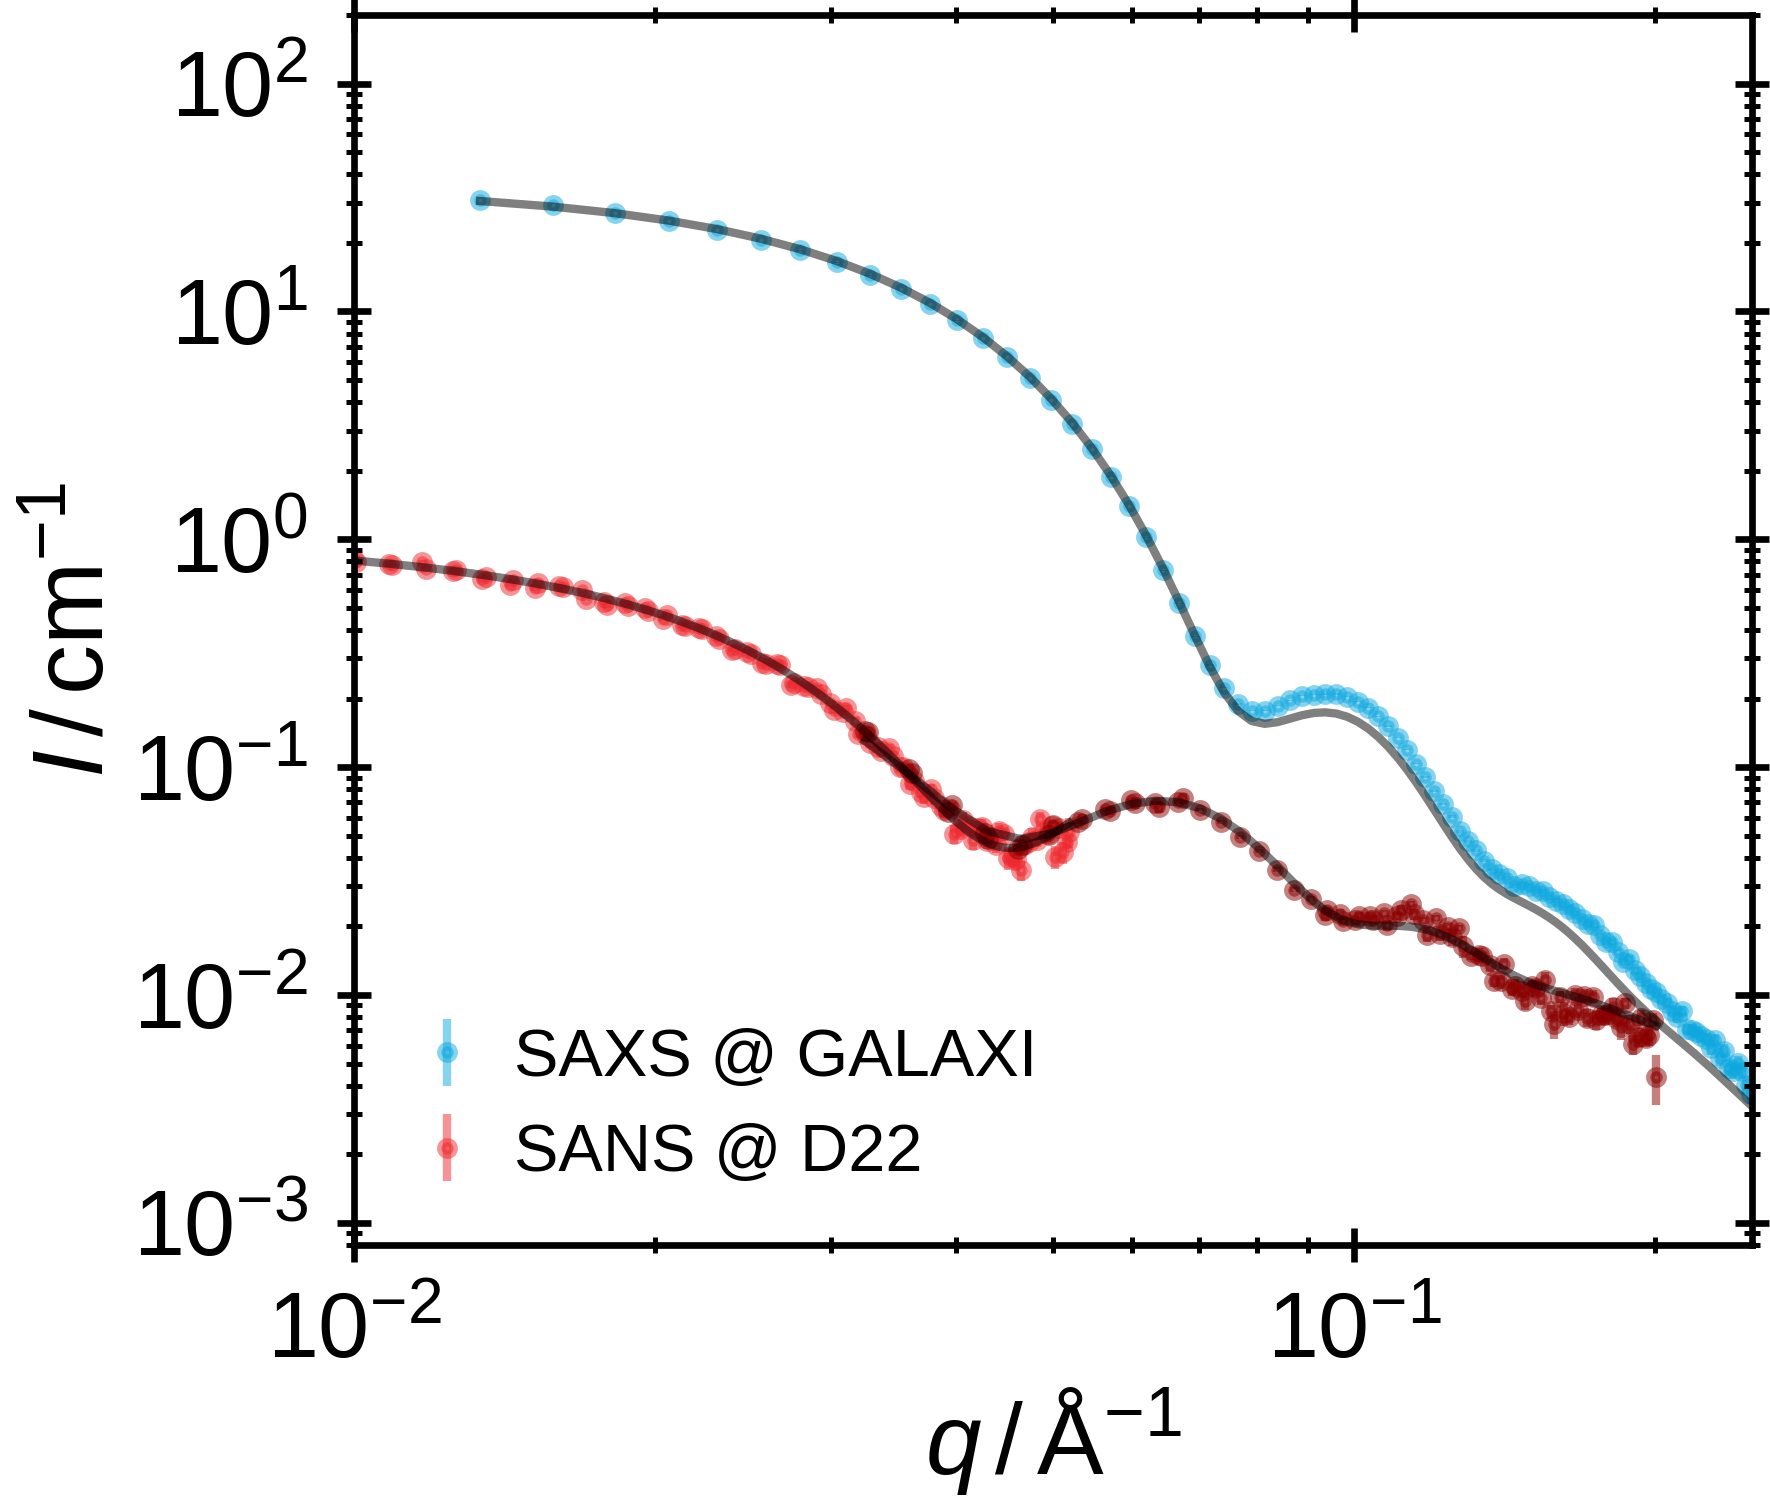
\includegraphics{monolayers_SAS_Ac_CoFe_C_SASSphereModelFit}
      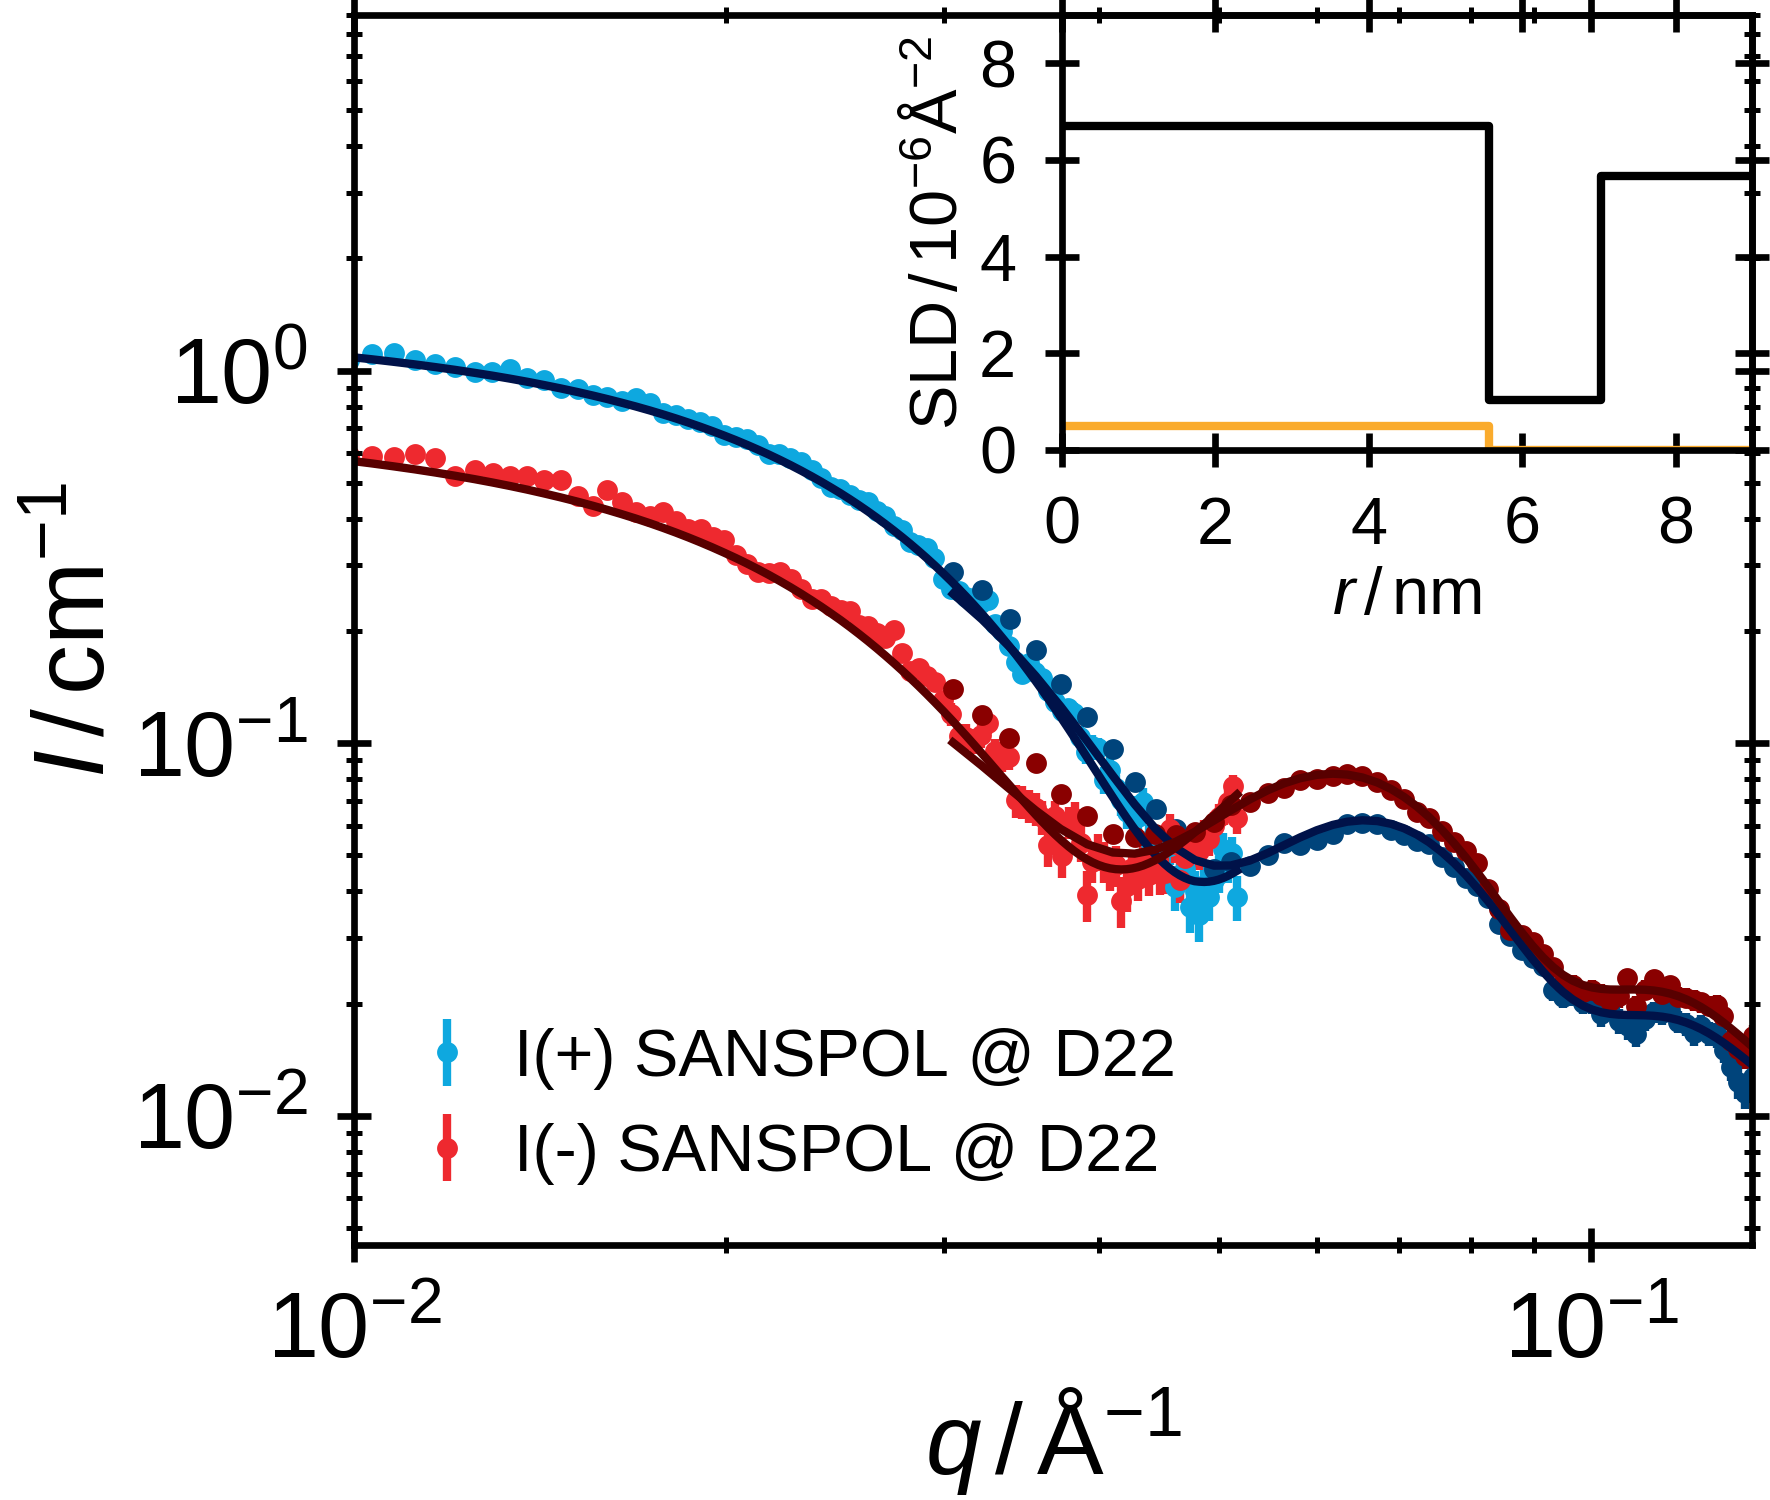
\includegraphics{monolayers_SAS_Ac_CoFe_C_SANSPOLSphereModelFit}
      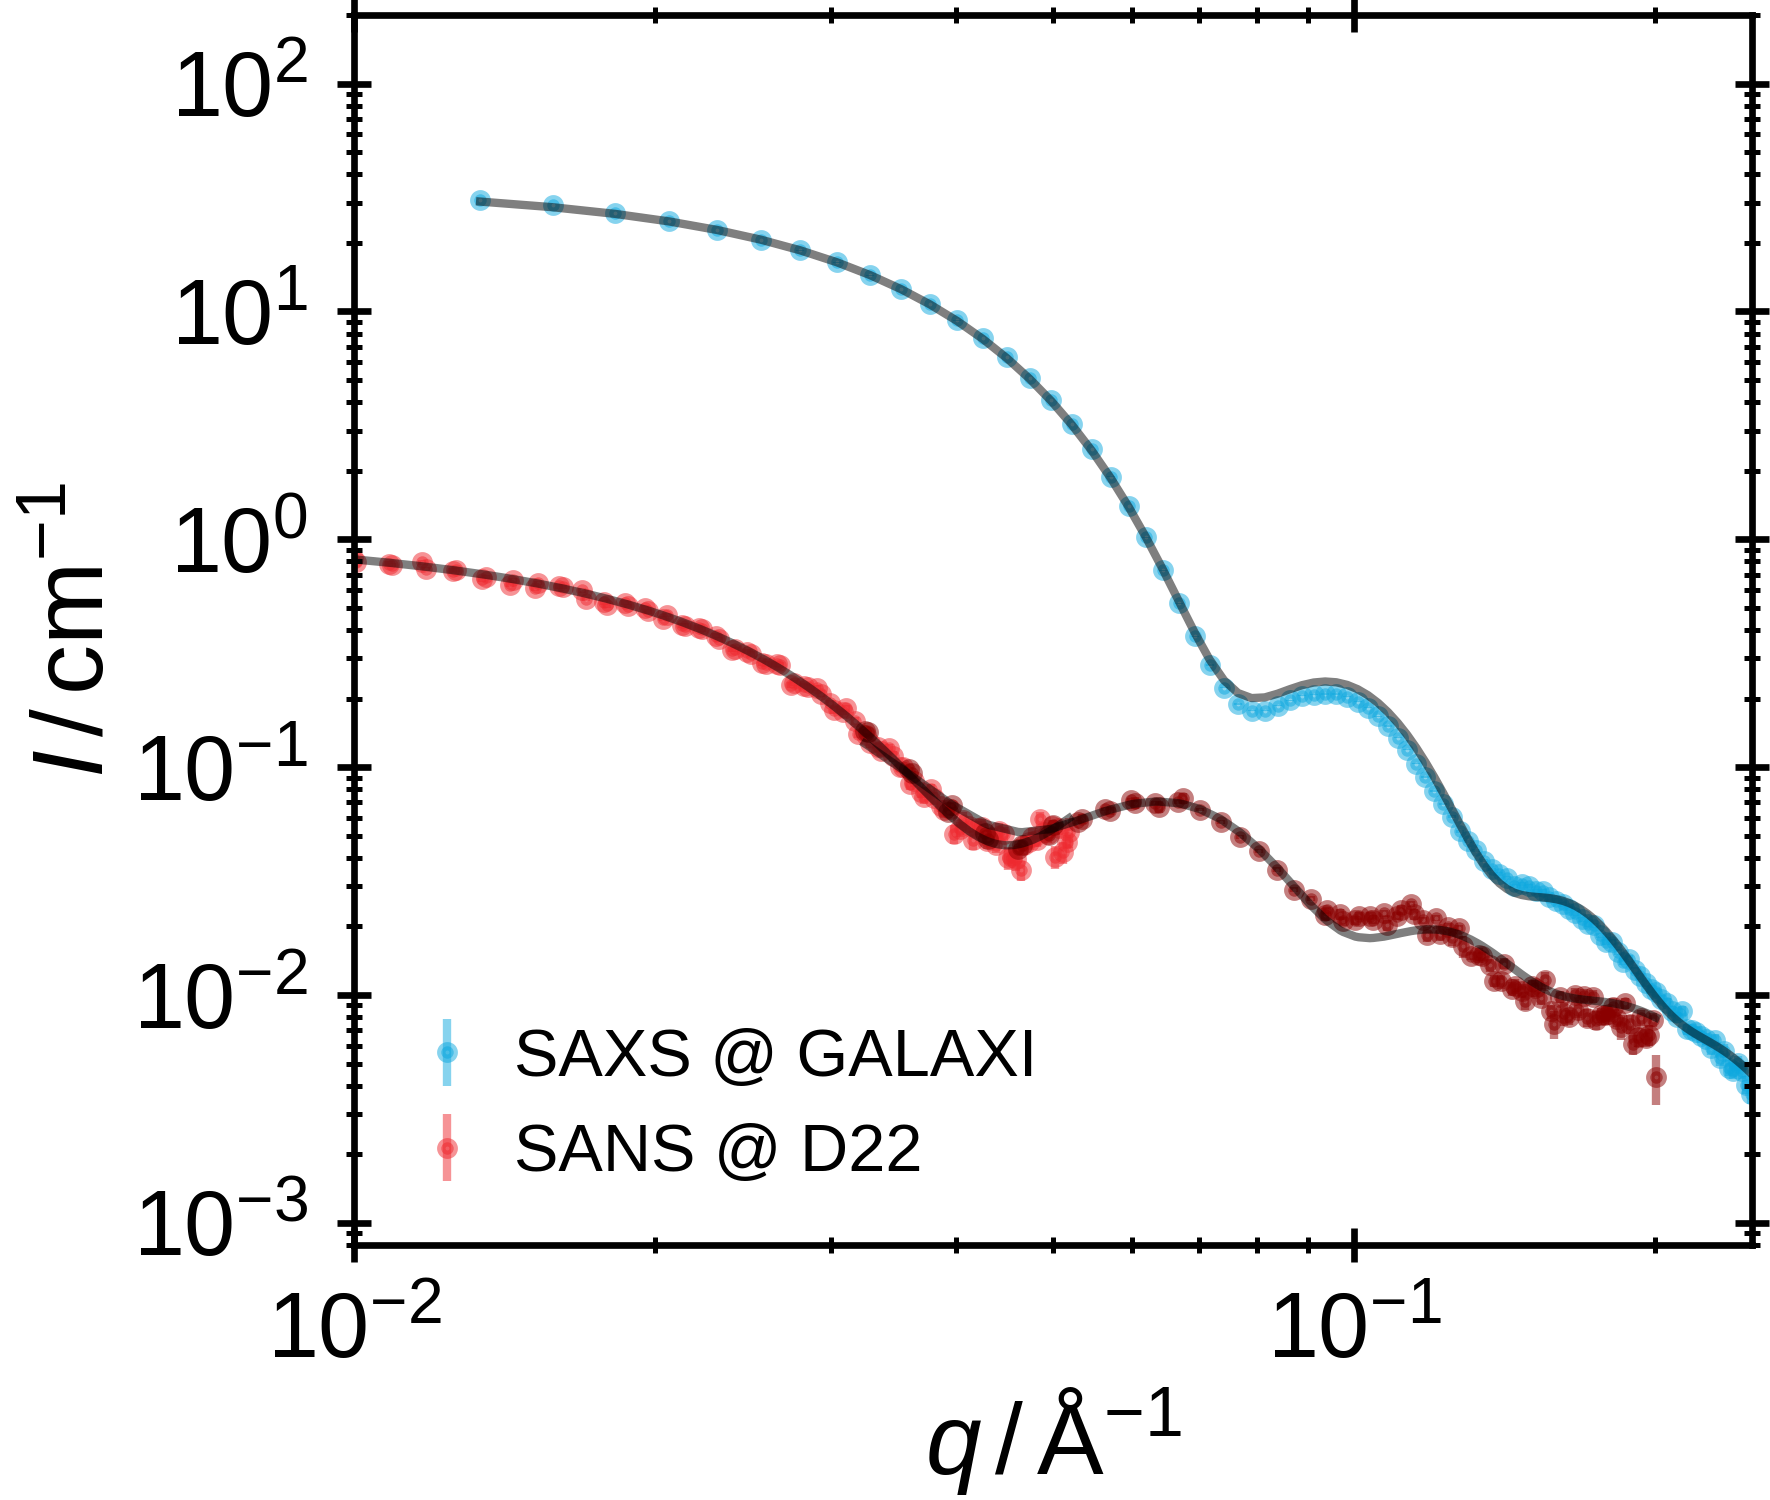
\includegraphics{monolayers_SAS_Ac_CoFe_C_SASCubeModelFit}
      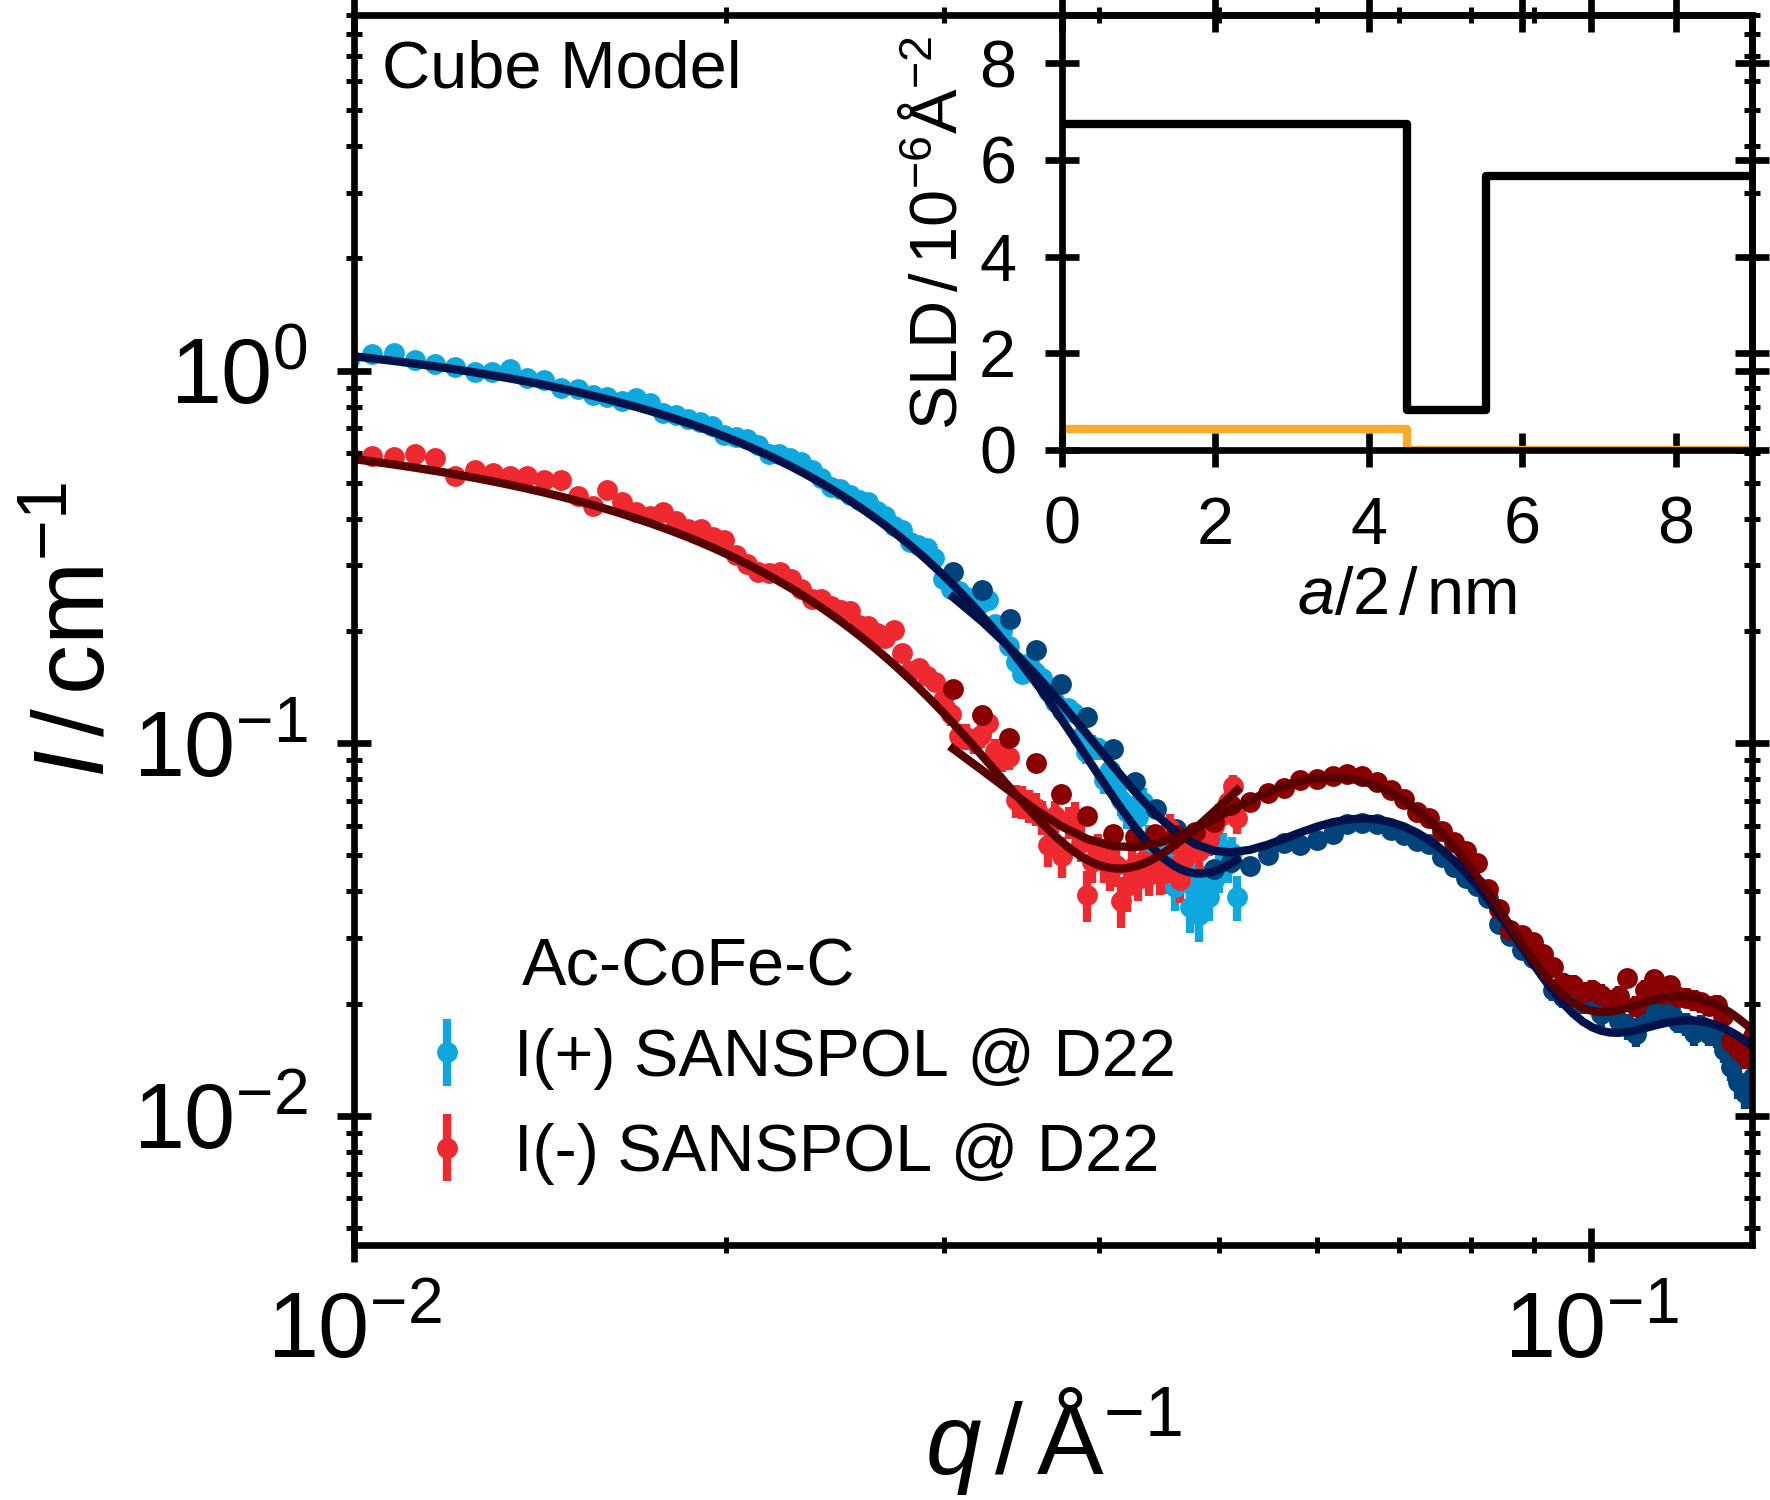
\includegraphics{monolayers_SAS_Ac_CoFe_C_SANSPOLCubeModelFit}
      \caption{\label{fig:monolayers:nanoparticle:sas:SphereCubeFit}Best sphere (upper) and cube model (lower) fit to the same SAS data of Ac-CoFe-C fitted in \reffig{fig:monolayers:nanoparticle:sas:AcOlCoFeC}. The left images show the fit of the nuclear structure for the two models, and the right the determination of the magnetic structure.}
    \end{figure}

    It's worthwhile to study the impact of the chosen shape model of the nanoparticle on the result of the magnetic scattering density.
    For this purpose, the simpler models of a perfect sphere and cube are fit additionally to the data of Ac-CoFe-C.
    These model provide a good reference point for the parameter values and as the models have one less parameter, they are additionally less prone to systematic errors in the fitting routine due to parameter correlations.
    The result of the cubic and spherical fit are shown in \reffig{fig:monolayers:nanoparticle:sas:SphereCubeFit} with the relevant parameters listed in \reftab{tab:monolayers:nanoparticle:sasSphereCubeFit}.

    \begin{table}[ht]
      \centering
      \caption{\label{tab:monolayers:nanoparticle:sasSphereCubeFit}Relevant parameters of the sphere and cube fit to the small-angle scattering data of Ac-CoFe-C, the complete set of parameters is found in \refapp{ch:appendix:modelparameters:monolayers:sas_olac_cofe_c}.}
      \begin{tabular}{ c | l | l }
          & Sphere & Cube \\
        \hline
        $R, \, a$
          & $5.56(2) \unit{nm}$
          & $9.01(2) \unit{nm}$\\
        $\sigma_R, \, \sigma_a$
          & $13.0(3) \,\%$
          & $10.7(2) \,\%$\\
        $D$
          & $1.46(4) \unit{nm}$
          & $1.03(4) \unit{nm}$\\
        $\rho_\mathrm{mag}^\mathrm{sans}$
          & $0.502(8) \cdot 10^{-6} \angstrom^{-2}$
          & $0.429(7) \cdot 10^{-6} \angstrom^{-2}$\\
        \hline
        $V_p$
          & $720(4) \unit{nm^{3}}$
          & $731(3) \unit{nm^{3}}$\\
        $M^\mathrm{sans}$
          & $172(3) \unit{kAm^{-1}}$
          & $147(2) \unit{kAm^{-1}}$\\
        \hline
      \end{tabular}
    \end{table}

    It's clearly visible by looking at the SAXS data that the spherical model underestimates the intensity of the first order peak, while the cube model overestimates it, whereas the superball was able to adjust in between.
    The determined particle volume varies only weakly from the specific choice of the model and therefore the model has only a minor effect on the rescaling procedure that is applied to the vibrating sample magnetometry data.
    From SANSPOL, it is visible that parameters such as the shell thickness, particle magnetization, as well as the particle concentration (listed in complete parameter set in \refapp{ch:appendix:modelparameters:monolayers:sas_olac_cofe_c}), are stronger affected by the choice of model in the fitting process.
    This becomes especially visible in the observation that the cube model estimates a smaller shell thickness and magnetization, whereas the sphere model suggests values that are a magnitude of $30 - 50 \unit{\%}$ higher.

    \begin{figure}[tb]
      \centering
      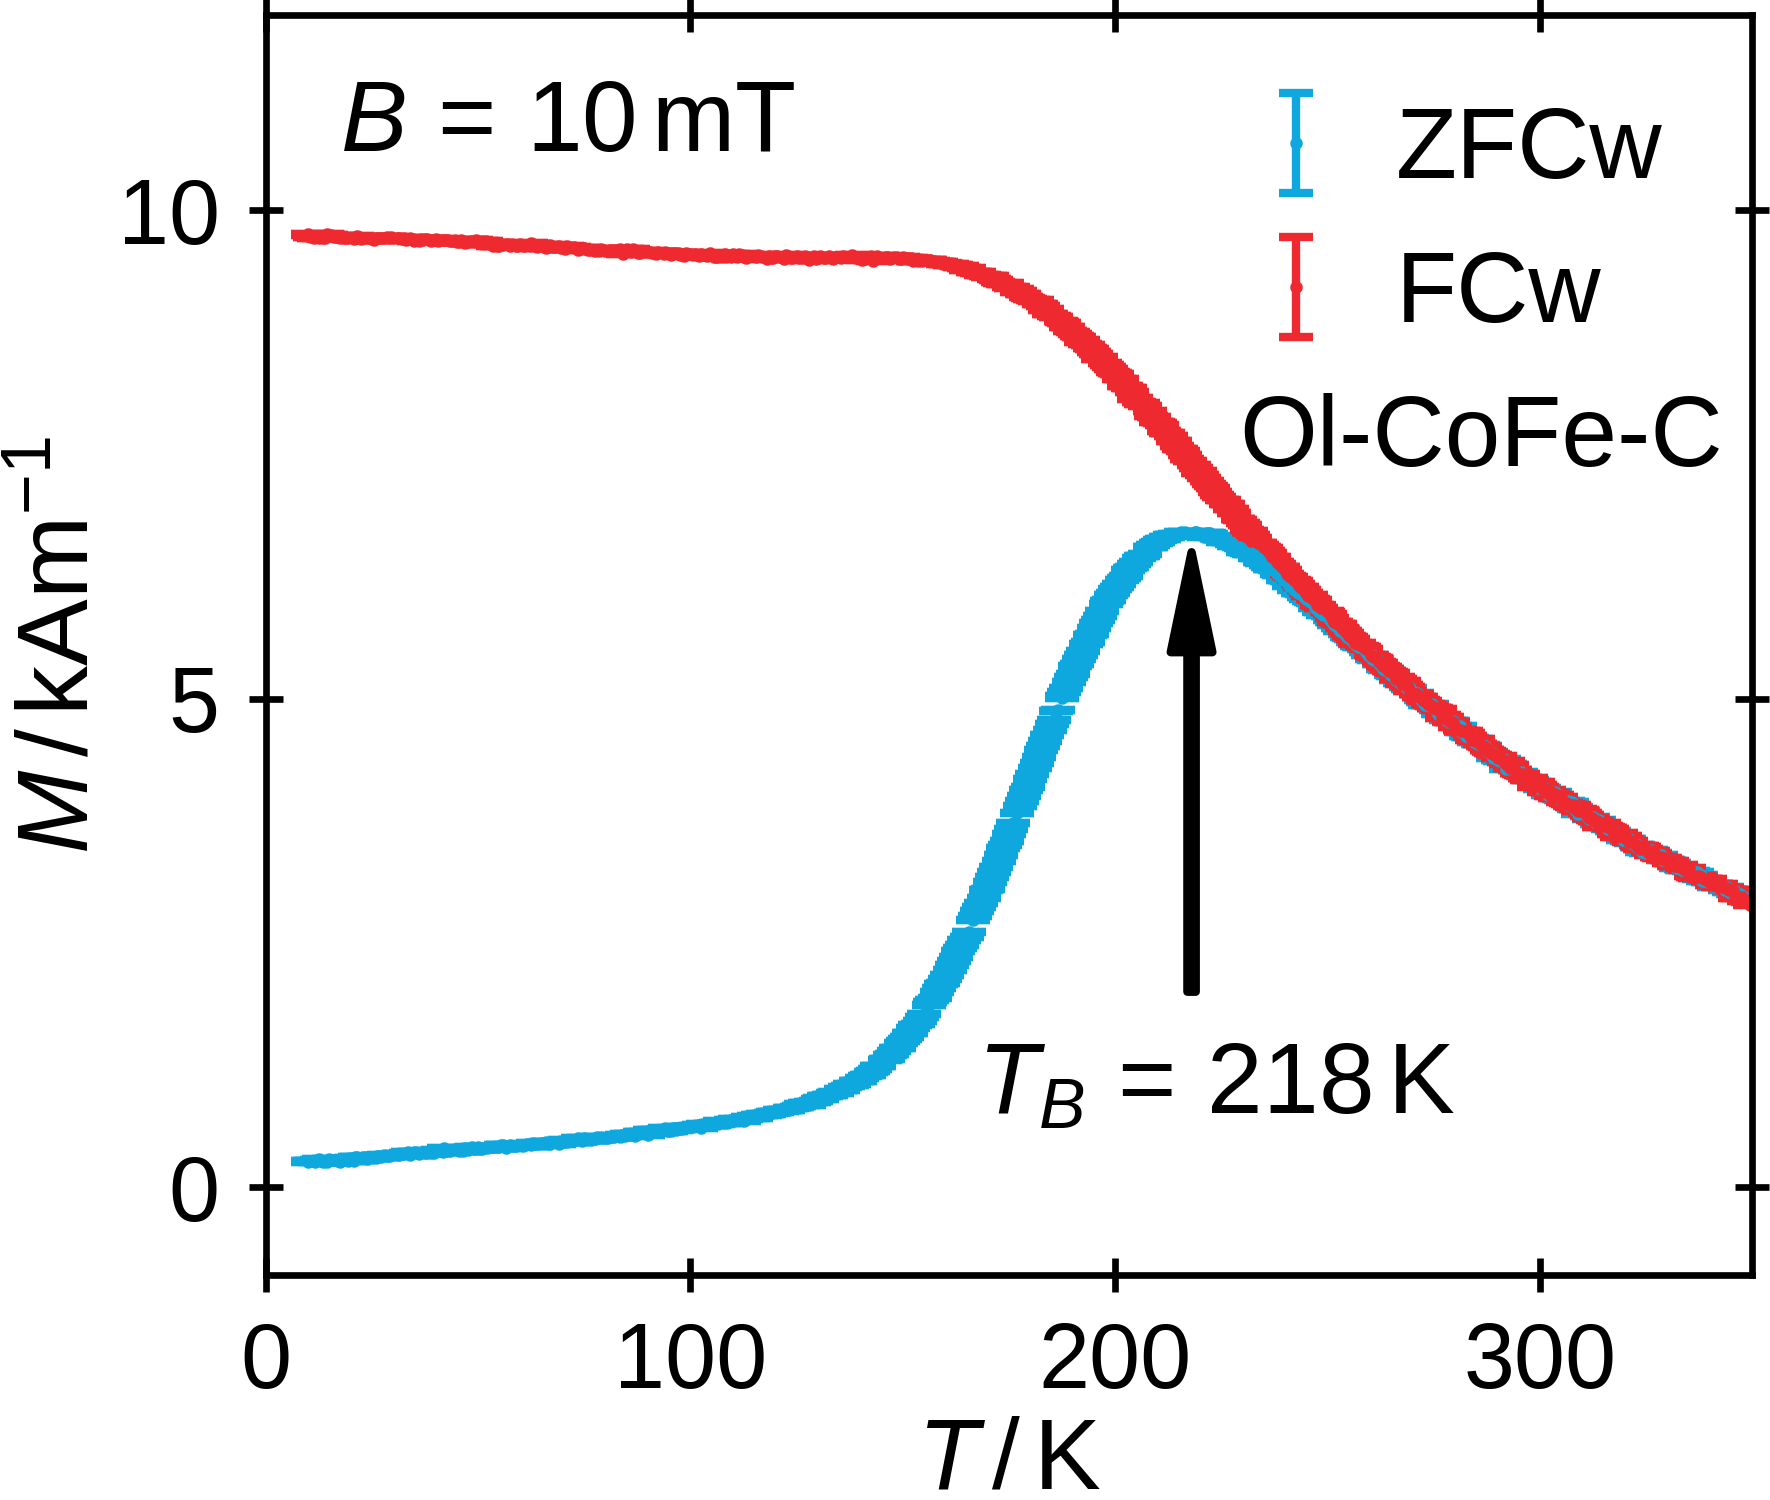
\includegraphics{monolayer_PPMS_ZFC_FC_ML_Ol_CoFe_C}
      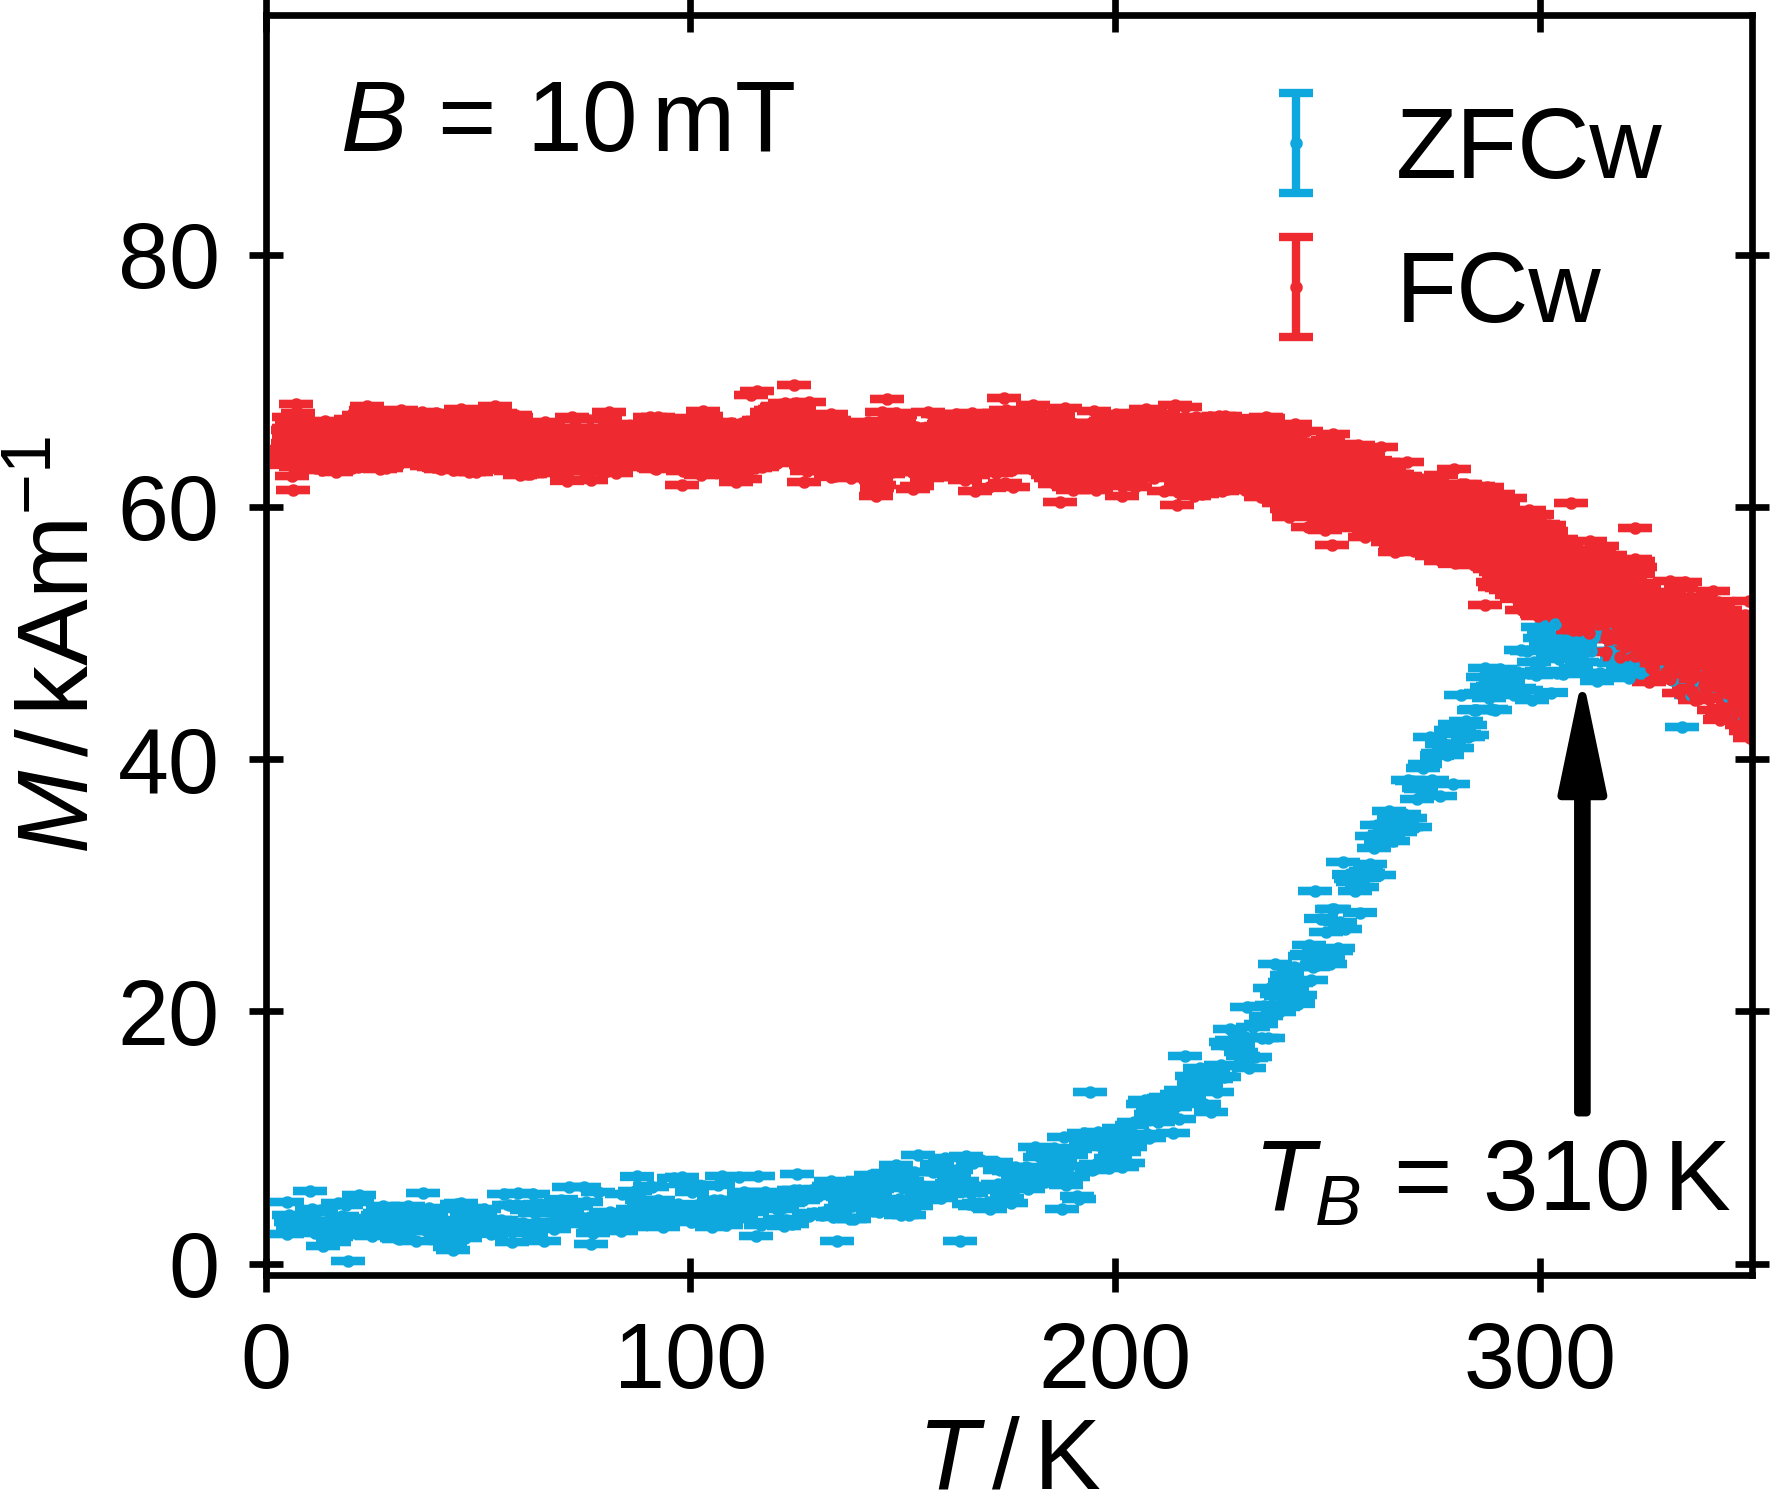
\includegraphics{monolayer_PPMS_ZFC_FC_ML_Ac_CoFe_C}
      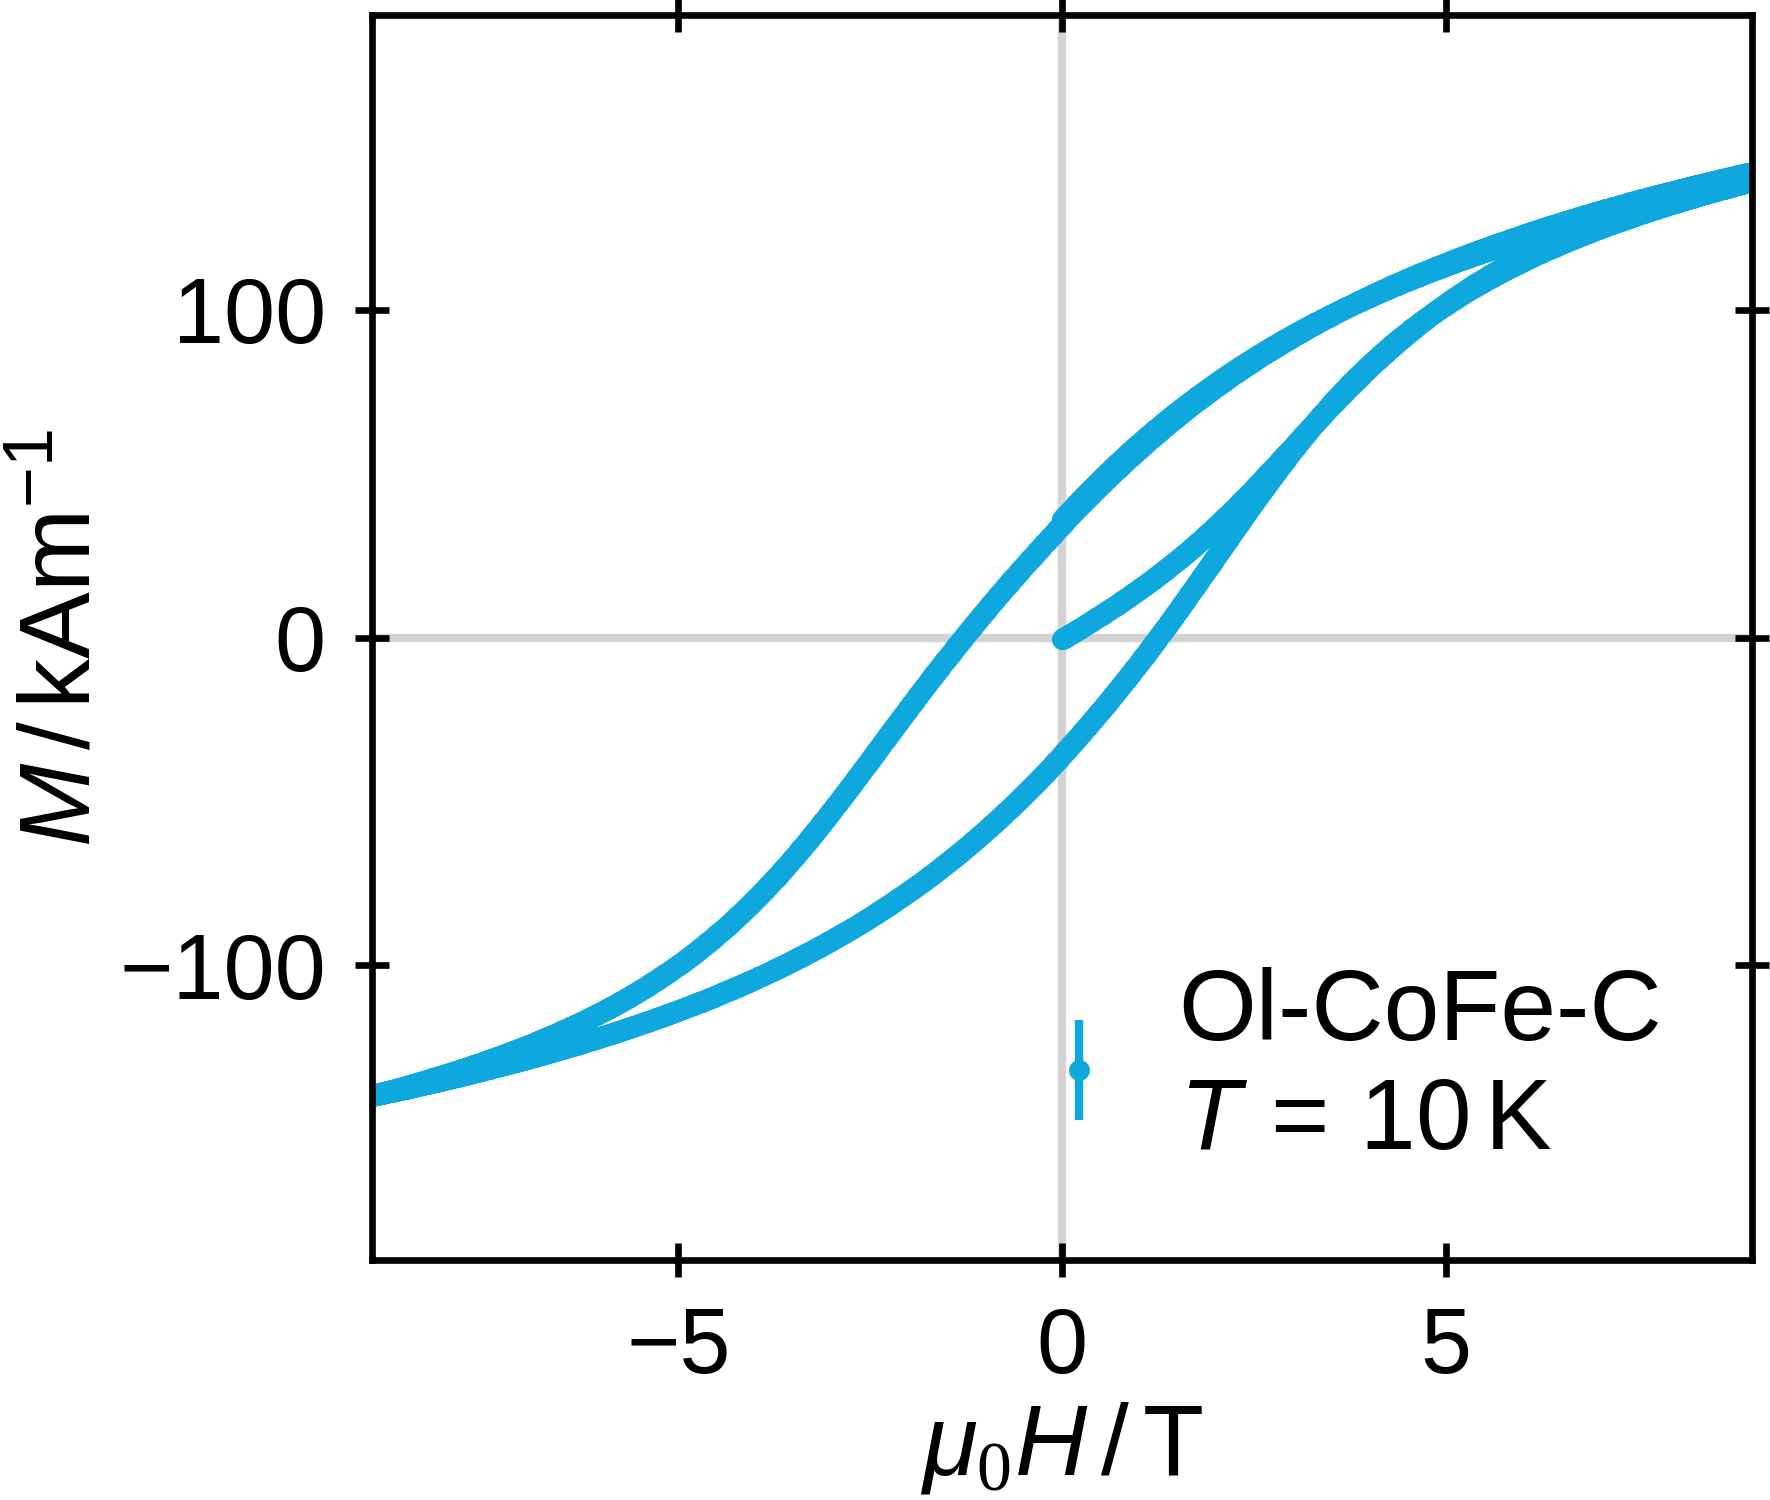
\includegraphics{monolayer_VSM_10K_Ol_CoFe_C}
      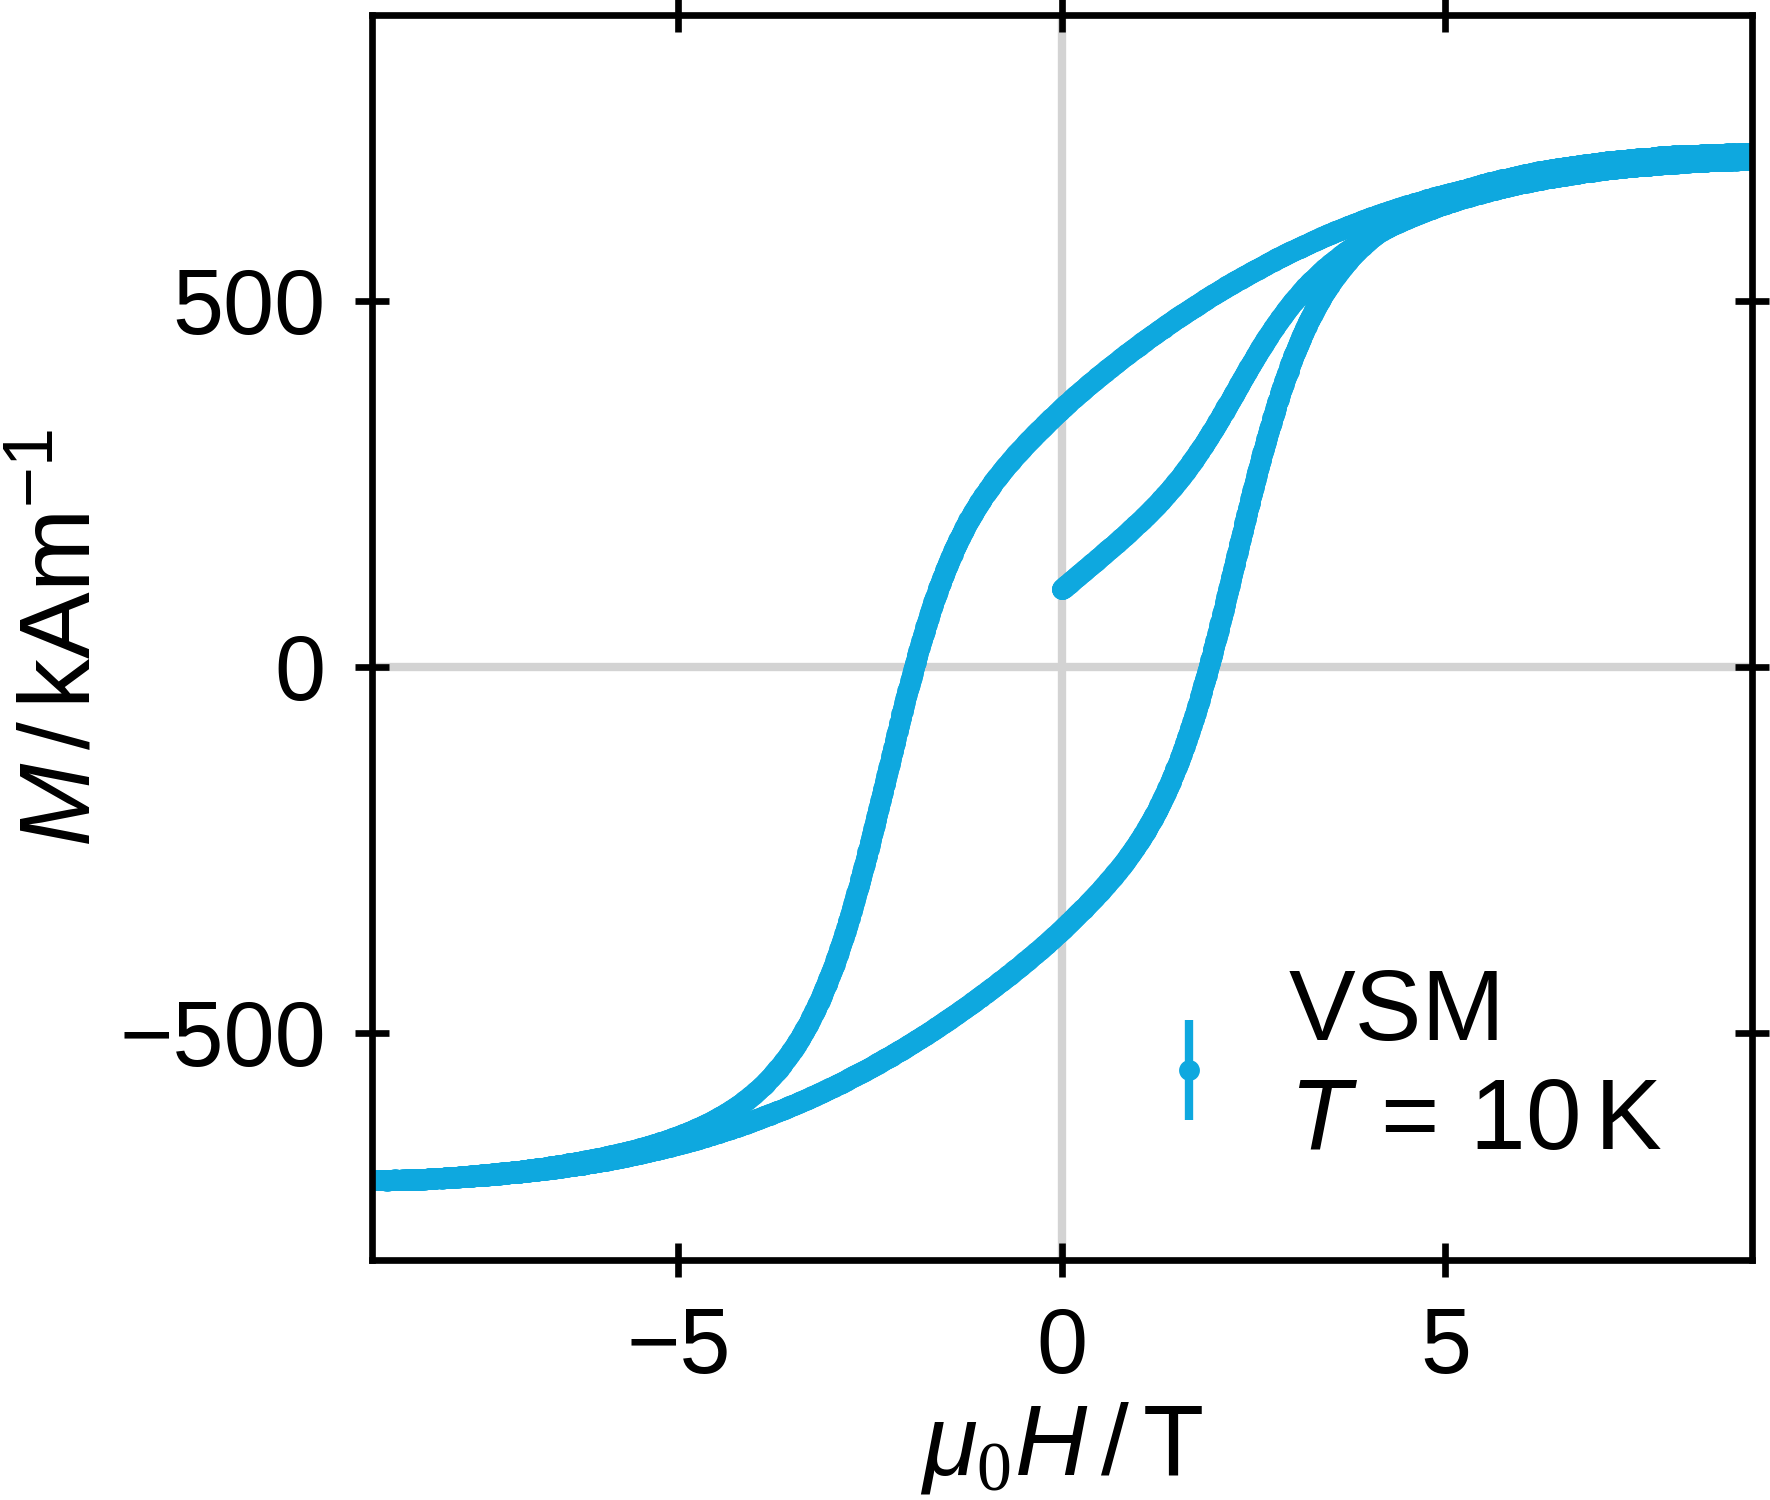
\includegraphics{monolayer_VSM_10K_Ac_CoFe_C}
      \caption{\label{fig:monolaye rs:nanoparticle:vsm10K}Low temperature hysteresis measurement of frozen Ol-CoFe-C (left) and Ac-CoFe-C (right) using the same samples as in \reffig{fig:monolayers:nanoparticle:vsm}.}
    \end{figure}

    To study the samples further, the nanoparticles are measured in VSM at varied temperatures down to $10 \unit{K}$, where the N\'eel relaxation of the superspin moment is suppressed and the blocked single-domain particle is observed.
    The magnetometry data is rescaled using the same factors that were determined at room temperature with the SAXS superball volume and Langevin fit.
    Both hysteresis are given in \reffig{fig:monolaye rs:nanoparticle:vsm10K} and show a large coercivity, where the coercive field for Ol-CoFe-C is at $1.2 \unit{T}$ and for Ac-CoFe-C at $1.9 \unit{T}$, which is the typical range that is also in literature for cobalt ferrite nanoparticles.
    From the temperature dependent magnetization measurements, the blocking temperature of the two particle batches can be estimated, which is $218 \unit{K}$ for Ol-CoFe-C and $314 \unit{K}$ for Ac-CoFe-C.
    % Zitate Nanoparticle Koerzitivfelder
    Additionally, Ol-CoFe-C shows an exchange bias effect, when the hysteresis is measured after cooling in a strong magnetic field such as shown by the red curve, which was obtained after cooling the sample in a $1 \unit{T}$ field.
    %Discuss Exchange Bias Effect

    \begin{figure}[tb]
      \centering
      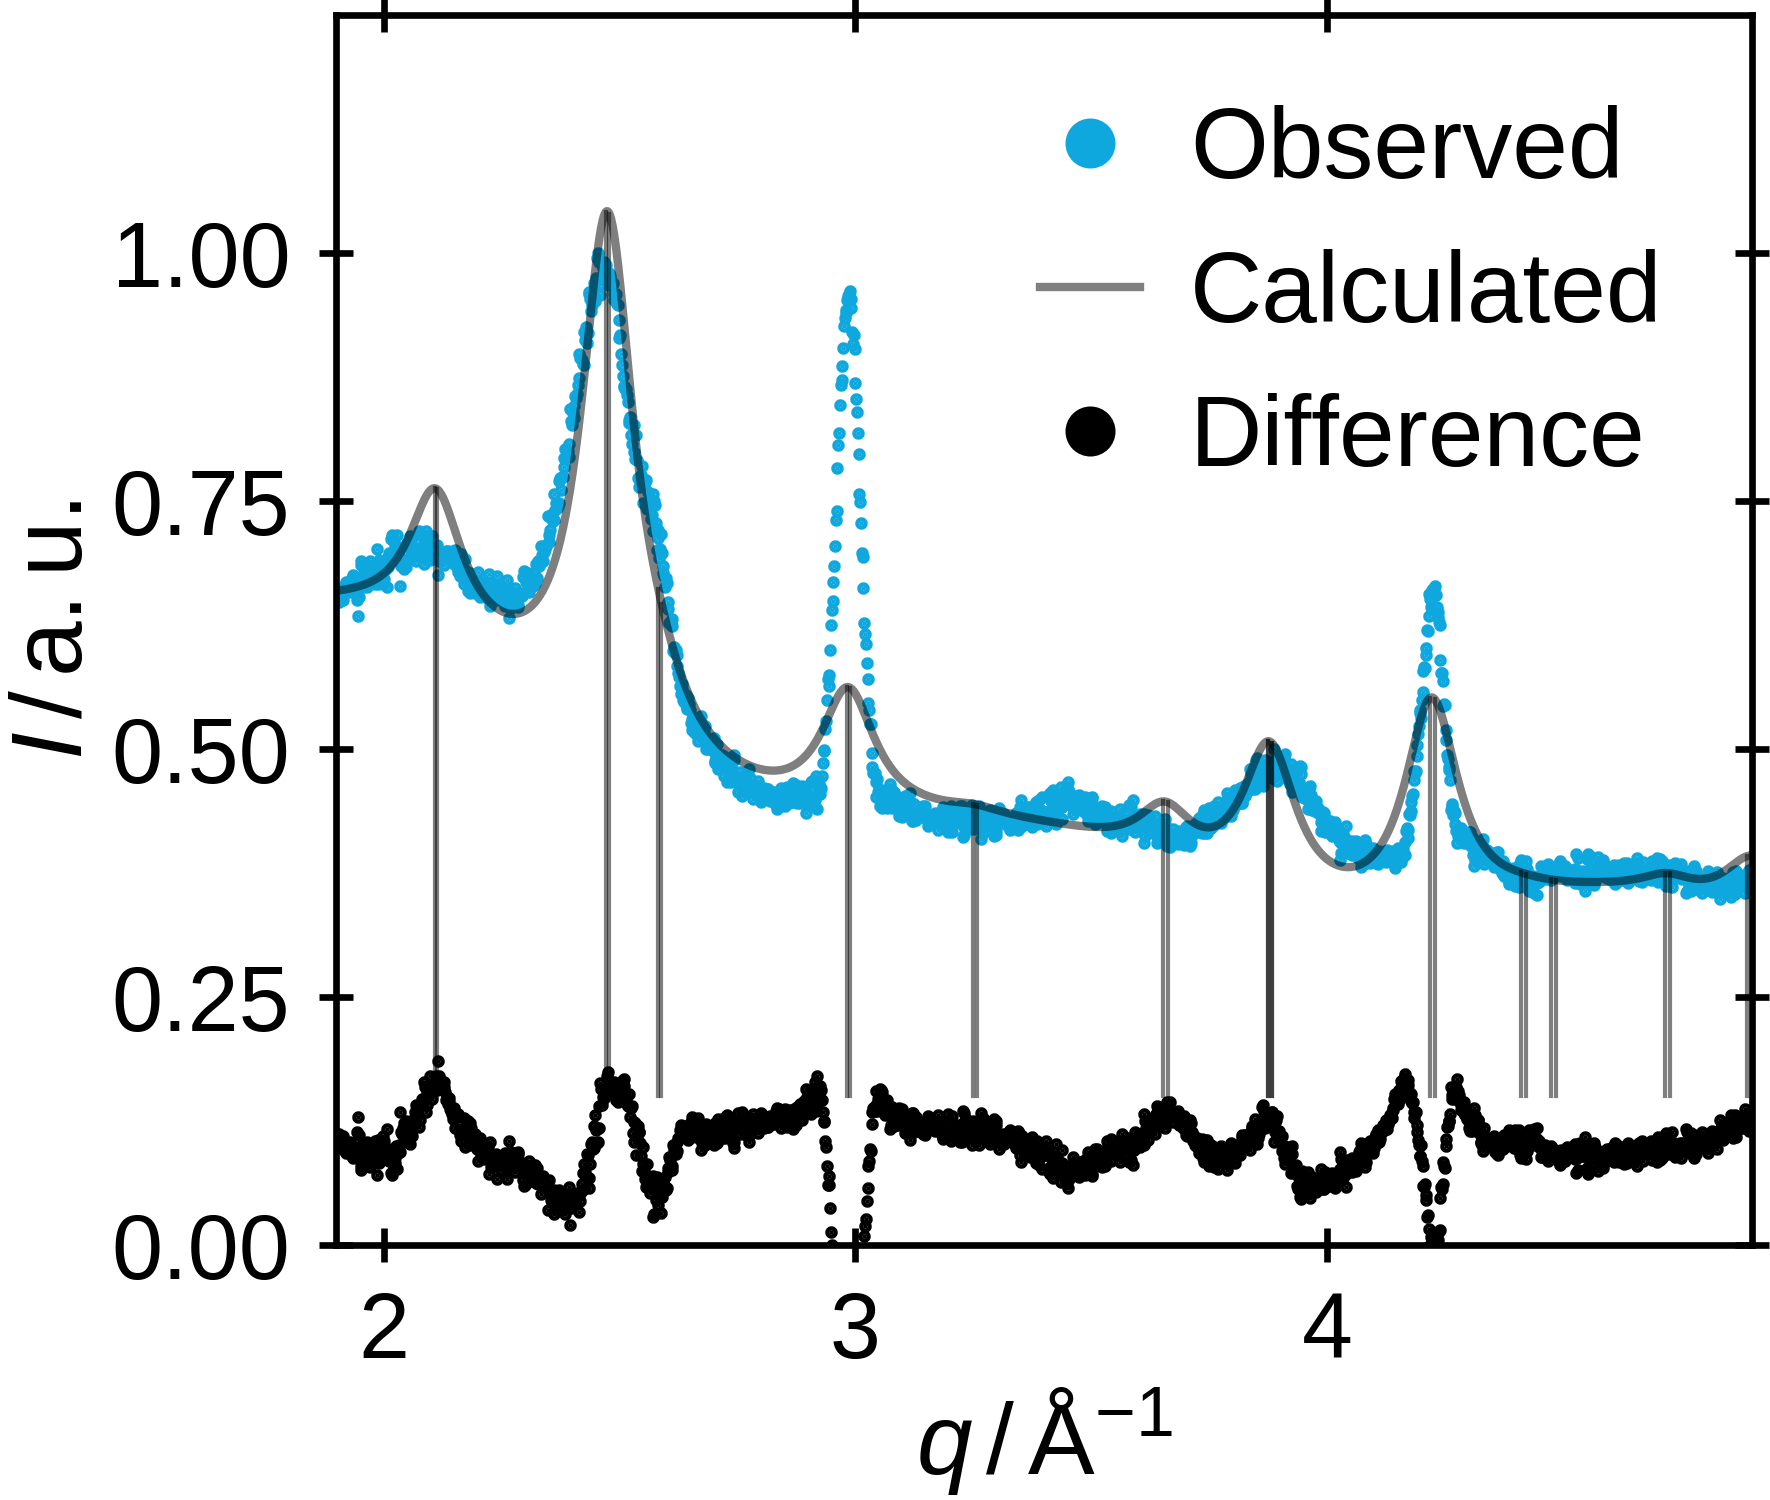
\includegraphics{monolayer_XRD_Ol_CoFe_C}
      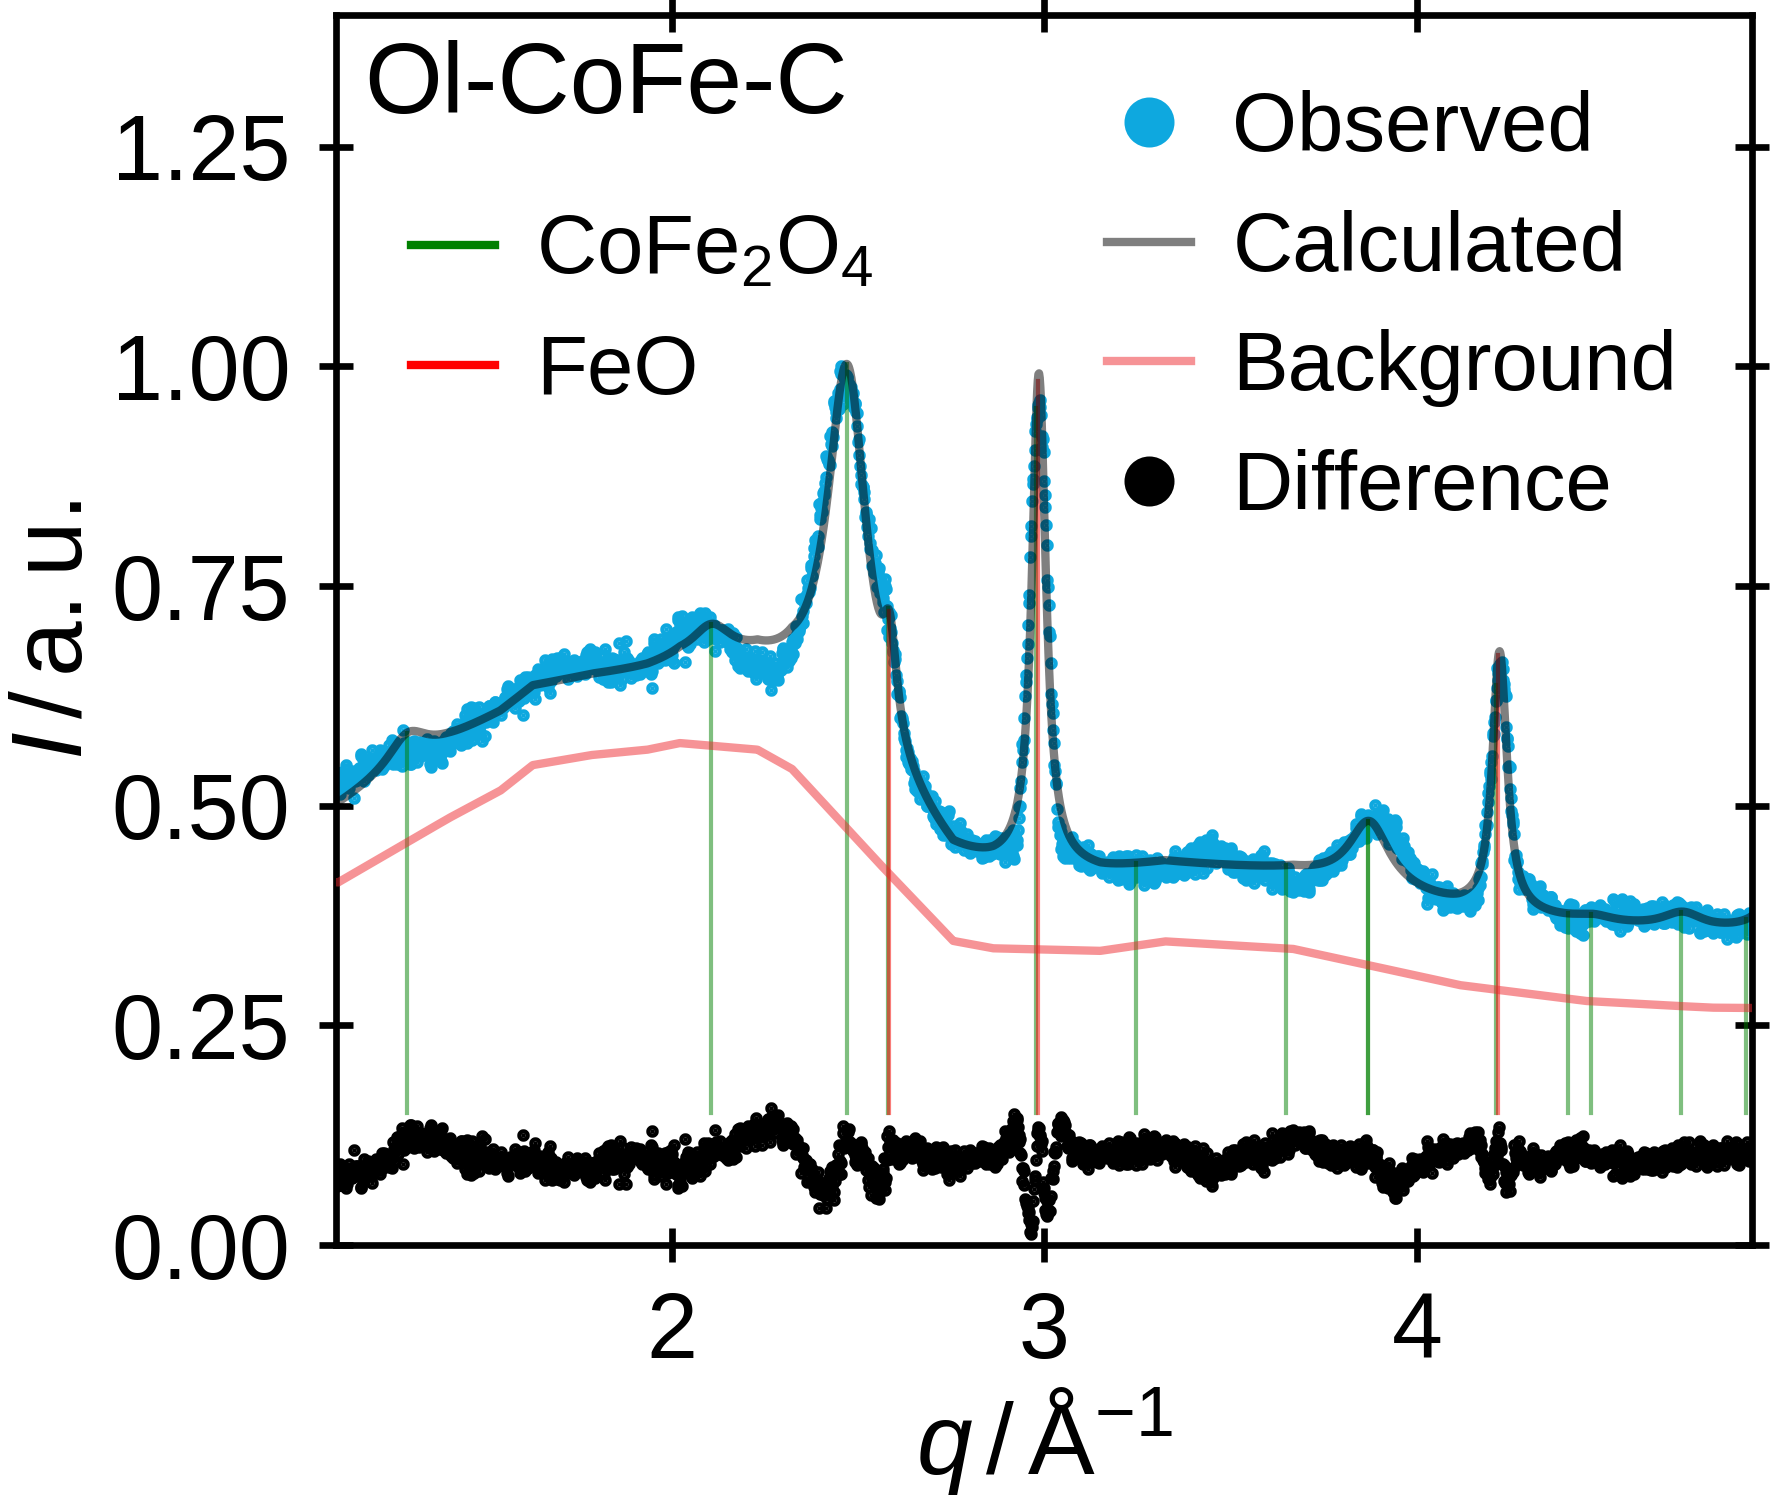
\includegraphics{monolayer_XRD_CoFe2O4WustiteFit_Ol_CoFe_C}
      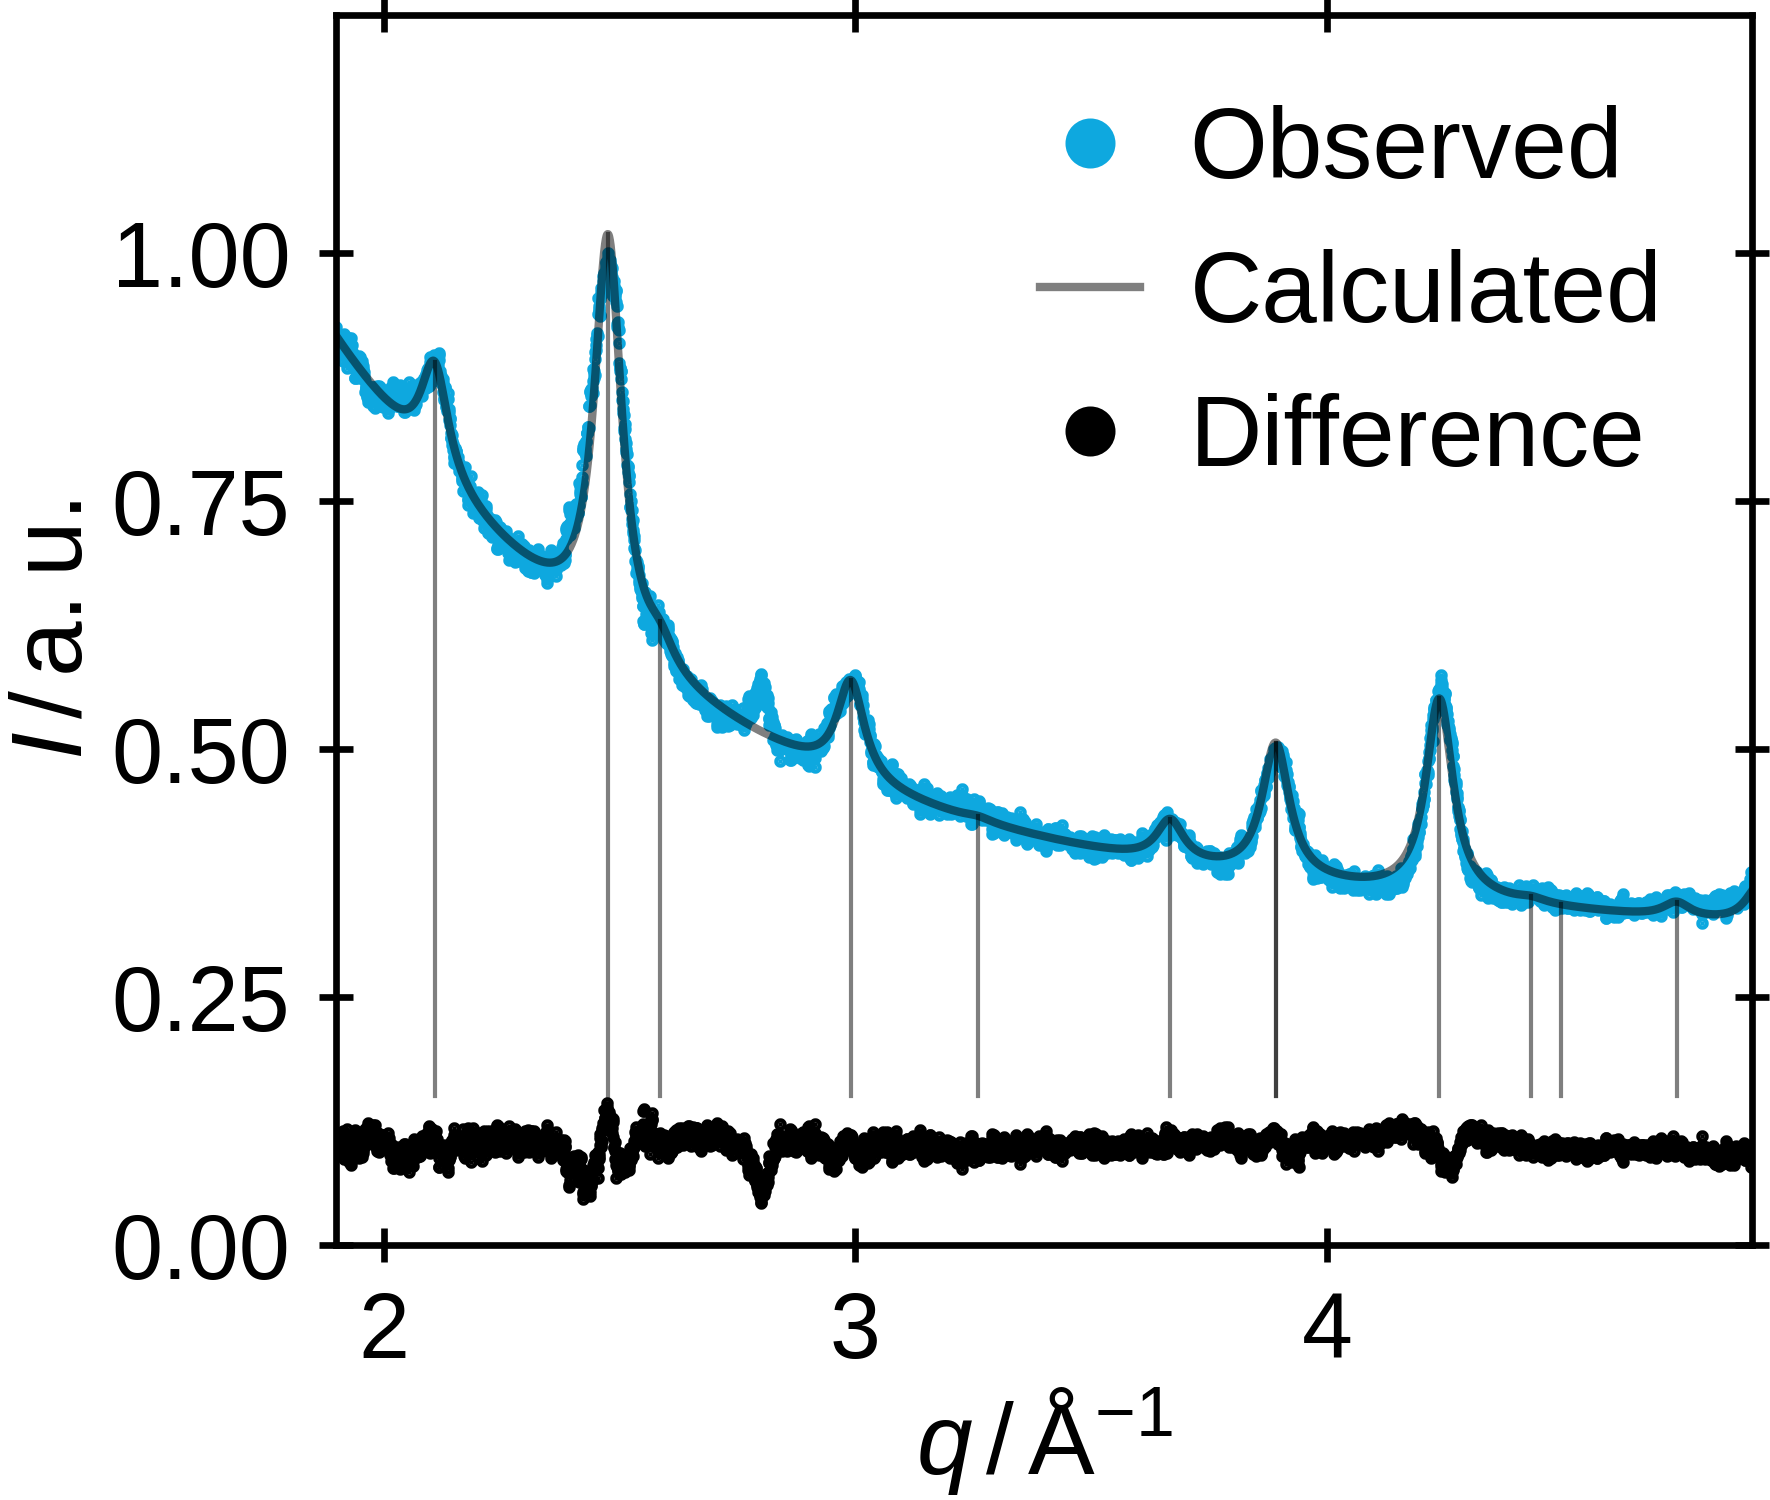
\includegraphics{monolayer_XRD_Ac_CoFe_C}
      \caption{\label{fig:monolayers:nanoparticle:xrd}X-ray diffraction of Ol-CoFe-C (upper left) and Ac-CoFe-C (lower left) with a Rietveld refinement assuming an inverse spinell structure. Additionally, Ol-CoFe-C was refined assuming a combination of an inverse spinell phase and a w\"ustite phase (upper right).}
    \end{figure}

    An explanation for the especially weak magnetic properties of the oleate synthesized particles and the exchange bias effect is found in literature by considering a second phase in the particle \cite{Bodnarchuk_2009_Excha, Wetterskog_2013_Anoma}.
    Instead of pure phased cobalt ferrite particles, core-shell particles with an w\"ustite core are obtained during the oleate synthesis due to the reductive environment of the synthesis.
    This is confirmed when looking at X-ray diffraction (XRD) data shown in \reffig{fig:monolayers:nanoparticle:xrd}

    The XRD data was measured in cooperation with the group of Daniel Nižňanský from the Department of Inorganic Chemistry at the Charles University in Prague, where the experimental details are found in \refapp{app:additionalExperimentalTechniques:xrd}.
    For both diffraction data sets a Rietveld analysis was performed using the FullProf Suite \cite{Rodriguez_1993_Recen}, where the expected inverse spinell structure of cobalt ferrite (space group Fd$\bar{3}$m, No. 227) was fitted.
    The order of adding parameters to the refinement was in all cases the same, where first the global parameters as the scale factor and background are estimated, and then the lattice parameter, peak shape and temperature displacement parameters are varied.
    The detailed list of the Rietveld refinement can be found in \refapp{ch:appendix:modelparameters:monolayers:xrd_olac_cofe_c}.
    The particles from acetylacetonates are reasonably well fitted by the structure model of \ch{CoFe2O4} with a $\chi^2 \eq 2.0$.
    On the other hand, Ol-CoFe-C can not be fitted well by assuming a single phase model only as visible in the upper left figure of \reffig{fig:monolayers:nanoparticle:xrd}.
    The relative intensity of the peaks do not match well and the reflex of the oleate nanoparticle is especially too strong around $q \eq 3 \unit{\angstrom^{-1}}$.
    And indeed, including a w\"ustite phase (space group Fm3m, No. 225) in the Rietveld analysis greatly improves the model as shown in the upper right image of \reffig{fig:monolayers:nanoparticle:xrd} and reduce the $\chi^2 \eq 13.1$ from only the single phase fit to $\chi^2 \eq 3.6$.
    The shown structure models neglect the cubic shape of the particles and possibly preferred orientation in the sample as the model is kept at a minimum of parameters for comparison.
    Also some temperature displacement parameters have not been fitted in the analysis but kept at $0$, as they tend to diverge to nonphysical negative values, when they are included in the analysis, as they try to absorb systematically missing parameters of the model.

    Additionally to providing information about the phases of the nanoparticles, the Rietveld analysis provides information about the average size of the crystallites $L$ in the sample.
    This is typically obtained via the Scherrer equation
    \begin{equation}
      L \eq \frac{K \lambda}{\beta \cos(\theta)},
    \end{equation}
    where $\lambda$ is the X-ray wavelength, $\beta$ the breadth of a peak, $\theta$ the scattering angle and $K$ the shape factor, which depends on the crystal shape, the definition of what is taken as peak breadth and the reflex indices \cite{Langford_1978_Scher}.
    In FullProf, $K$ is set to 1 and $\beta$ is determined from the pseudo-Voigt line profile according to the formula given by De Keijser \cite{DeKeijser_1982_Useof}.
    The average crystallite size is determined to $L \eq 5.8 \unit{nm}$ for Ac-CoFe-C and $L_{\ch{CoFe2O4}} \eq 2.0 \unit{nm}$, $L_{\textsf{w\"ustite}} \eq 10.9 \unit{nm}$ for the two phases of Ol-CoFe-C.
    The value of Ac-CoFe-C is considerably smaller than the actual particle size determined by electron microscopy and small angle scattering.
    This can be linked to possible structural disorder in the particles that systematically reduces the coherent scattering, which could also be the reason as to why the magnetization of the particles is still considerably smaller than the bulk magnetization of typical cobalt ferrite or maghemite even though it has a pure phase.

    In summary, the two heating up syntheses of cobalt ferrite nanocubes that are presented here provide a trade-off in homogeneous shape vs. phase purity and strong magnetism.
    Both syntheses yield cubic particles in the size of approximately $10 \unit{nm}$.
    While the cubes from the oleate synthesis are more homogeneous in shape but has a core-shell phase with weak magnetic properties, the cubes from the acetylacetonates synthesis have a pure phase with stronger magnetic properties but a broader size distribution.
    This has been shown by using complementary experimental techniques that give a mutual and reliable picture of the global size properties.
    In the following both batches will be used to study the properties of self-assembled long range ordered monolayers, where Ol-CoFe-C is used to study the parameters for preparing high quality monolayers, Ac-CoFe-C is used to study the collective magnetism of long range ordered monolayers.
\end{document}